%%%%%%%%%%%%%%%%%%%%%%%%%%%%%%%%%%%%%%%%%%%%%%%%%%%%%%%%%%%%%%%%%%%%%%%%%%%%%%%%
%2345678901234567890123456789012345678901234567890123456789012345678901234567890
%        1         2         3         4         5         6         7         8

%\documentclass[letterpaper, 10 pt, conference]{ieeeconf}  % Comment this line out if you need a4paper

\documentclass[letterpaper, 10pt, conference]{ieeeconf}      % Use this line for a4 paper

\IEEEoverridecommandlockouts                              % This command is only needed if 
                                                          % you want to use the \thanks command

\overrideIEEEmargins                                      % Needed to meet printer requirements.

%In case you encounter the following error:
%Error 1010 The PDF file may be corrupt (unable to open PDF file) OR
%Error 1000 An error occurred while parsing a contents stream. Unable to analyze the PDF file.
%This is a known problem with pdfLaTeX conversion filter. The file cannot be opened with acrobat reader
%Please use one of the alternatives below to circumvent this error by uncommenting one or the other
%\pdfobjcompresslevel=0

% See the \addtolength command later in the file to balance the column lengths
% on the last page of the document

% The following packages can be found on http:\\www.ctan.org
\usepackage{graphics} % for pdf, bitmapped graphics files
%\usepackage{epsfig} % for postscript graphics files
%\usepackage{mathptmx} % assumes new font selection scheme installed
%\usepackage{times} % assumes new font selection scheme installed
%\usepackage{amsmath} % assumes amsmath package installed
%\usepackage{amssymb}  % assumes amsmath package installed

\usepackage{graphicx}
\graphicspath{ {./graphics/} }

\usepackage{xcolor}
\usepackage{subcaption}
\captionsetup{font=footnotesize}

\newcommand{\ph}[1]{{\textbf{#1}:}} % paragraph header
\newcommand{\todo}[1]{{\color{red} #1 }} % Tasks to do
\newcommand{\inst}[1]{{\color{orange} #1 }} % instructions
% \newcommand{\kyon}[1]{{\color{blue} #1 }}
\newcommand{\rev}[1]{{\color{blue} #1 }} % Tasks to do --Previously BLUE
\newcommand{\comment}[1]{} 

\usepackage[normalem]{ulem}
\usepackage{url}
\usepackage{amsmath}
\usepackage{amsfonts}
\usepackage{amssymb}
\usepackage{soul}
\usepackage{textcomp}

\title{\LARGE \bf
Autonomous Spot: \\
Long-range Autonomous Exploration of \\Extreme Environments with Legged Locomotion
%NeBula Autonomy on Boston Dynamics \textsc{Spot} Robot: \\
%Enabling Autonomous Exploration of Extreme Environments% Title consideration:
% 1. People can easily search "Autonomous Spot" and the paper will appear
% 2. A 2-4 noun words to recall: like Autnomous Spot in Challenging environment
}


\author{Amanda Bouman$^{*2}$, Muhammad Fadhil Ginting$^{*1}$, Nikhilesh Alatur$^{*2}$, Matteo Palieri$^{1}$, \\
David D. Fan$^{1}$, Thomas Touma$^{2}$, Torkom Pailevanian$^{1}$, Sung-Kyun Kim$^{1}$, Kyohei Otsu$^{1}$,\\
Joel Burdick$^{2}$, Ali-akbar Agha-Mohammadi$^{1}$% <-this % stops a space
\thanks{$^*$ These authors contributed equally to this work.}
\thanks{$^{1}$ NASA Jet Propulsion Laboratory, California Institute of Technology, Pasadena, CA, USA,
     {\tt\small aliagha@jpl.nasa.gov}}%
\thanks{$^{2}$Department of Mechanical and Civil Engineering, Division of Engineering and Applied Science, California Institute of Technology, Pasadena, CA, USA,
         {\tt\small jwb@robotics.caltech.edu}}%
% \thanks{$^{3}$ Department of Electrical And Information Engineering, Polytechnic University of Bari, Bari, Italy}%
% \thanks{$^{4}$Department of Mechanical and Process Engineering, Institute of Robotics and Intelligent Systems, Swiss Federal Institute of Technology in Zurich, Zurich, Switzerland}%
}

\begin{document}
\maketitle
\thispagestyle{empty}
\pagestyle{empty}
%%%%%%%%%%%%%%%%%%%%%%%%%%%%%%%%%%%%%%%%%%%%%%%%%%%%%%%%%%%%%%%%%%%%%%%%%%%%%%%%
\begin{abstract}
This paper serves as one of the first efforts to enable large-scale and long-term autonomy using the Boston Dynamics Spot robot. 
Motivated by exploring extreme environments and in particular underground environments in the DARPA Subterranean Challenge, this paper pushes the boundaries of the state-of-practice in enabling legged robotic systems to accomplish real-world complex missions in relevant scenarios. 
In particular, we will discuss the behaviors and capabilities which emerge from the integration of the autonomy \rev{architecture}NeBula (Networked Belief-aware Perceptual Autonomy) with next-generation mobility systems.
We will discuss the \rev{hardware and software}challenges, and solutions in mobility, perception, autonomy, and wireless networking, as well as lessons learned and future directions. 
We demonstrate the performance of the proposed solutions on physical systems in real-world scenarios.
\rev{The proposed solution contributed}to winning 1st place in the 2020 DARPA Subterranean Challenge, Urban Circuit.
\end{abstract}
%Video: Experimental results are available at ... 

%%%%%%%%%%%%%%%%%%%%%%%%%%%%%%%%%%%%%%%%%%%%%%%%%%%%%%%%%%%%%%%%%%%%%%%%%%%%%%%%
% \section{Instructions}
% \ph{Paragraph header} 
% \inst{Please start \uline{every single paragraph} with a paragraph header, summarizing the intention of that paragraph. This is mainly for iterations during the paper preparation. We can remove most of them for the final report.

% Graphs are available here for modification : 
% \url{https://docs.google.com/presentation/d/1dja02gUoBeNuNW-aHb6CmwaFevmf-jXMHk02NYbL1Ok/edit?usp=sharing}
% }
% {\color{red}fadnik means Fadhil or Nikhilesh}

% General Flow of the paper
% Introduction
% Architecture -> philosopy NeBula
% Mobility manager -> locomotion include from BD coauthor from them and sensors
% State Estimation -> Spot Frontend
% Perception Aware Planning -> Perception Aware Planning to Face Forward ..
% Experimental Result
% Lesson Learned  and Future:
% Recovery,
% Maybe stairs

% Conclusions



%%%%%%%%%%%%%%%%%%%%%%%%%%%%%%%%%%%%%%%%%%%%%%%%%%%%%%%%%%%%%%%%%%%%%%%%
\section{Introduction}\label{sec:intro}
%%%%%%%%%%%%%%%%%%%%%%%%%%%%%%%%%%%%%%%%%%%%%%%%%%%%%%%%%%%%%%%%%%%%%%%%
\rev{Robotic and autonomous mapping and traversal of extreme environments under time constraints has a wide variety of real-world applications. 
They range from search and rescue after natural disasters \cite{Nagatani2013} over exploration of extreme planetary terrains \rev{\cite{ali-agu}, \cite{Taka2020JFR}, \cite{Husain2013}}to inspection of underground infrastructure in urban environments~\cite{Kolvenbach2020}.
%\rev{This paper discusses Team CoSTAR's synergistic approach of combining advanced quadrupedal locomotion and high-level autonomy in order to accomplish complex missions.}
%In this paper, we discuss how bridging advanced locomotion capabilities and autonomy can address such complex missions. 
%In this paper, we discuss how bridging advanced locomotion capabilities and autonomy can address such complex missions.
This paper discusses Team CoSTAR's synergistic approach of endowing a sophisticated legged platform with high-level autonomy in order to accomplish complex missions. We focus our research and development around real-world robotics scenarios. 
As such, the DARPA Subterranean (SubT) Challenge \cite{subt_webpage} presents us with the ideal setting to demonstrate the efficacy of our entire system architecture. 
The SubT challenge requires robot teams to rapidly explore, map, and search extreme underground environments in order to find objects of interest.
%\st{As a concrete mission,} we focus on the DARPA Subterranean (SubT) Challenge \cite{subt_webpage}, a robotic competition that targets one such mission to explore, map, and search extreme underground environments. 
%\rev{The complexity of these missions presents mobility challenges which impose constraints on the solution space.}
%From a mobility perspective, this mission imposes lots of constraints on the solution space.
%\rev{Various requirements imposed by elements of extreme environments include:}

Elements of these extreme environments dictate requirements that necessitate novel mobility capability development. These requirements include:
%Some conflicting requirements imposed by elements of such extreme environments are
1) sufficient payload capacity for sensing, autonomy, computation and communication, 2) endurance for long-duration, complex and spatially large (\texttildelow $km^2$) mission scenarios, 3) anthropomorphically analogous physical dimensions for traversing tight passages ($\geq$80cm), 4) advanced traversability capabilities for staircases, uneven terrain, obstacle laden surfaces and high-risk regions.}
%1) ability to carry a large-enough payload that can enable high-levels of sensing, autonomy, computing, and communication capabilities, 2) endurance for long-term missions (at least 1 hour) and large areal coverage (multi-kilometers in length), 3) to be small enough to go through passages as narrow as 80 cm in diameter, and 4) ability to traverse mobility-stressing features such as stairs, uneven terrains and obstacle-laden areas with high-risk regions. 

\begin{figure}[t!]
  \centering
  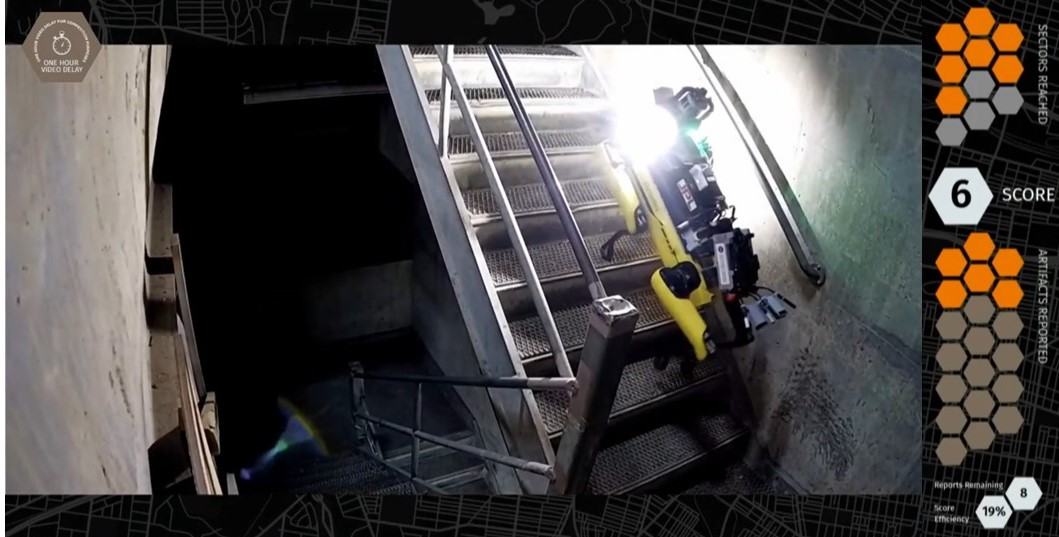
\includegraphics[width=0.5\textwidth]{graphics/spot_cover_ver1.jpg}
  \caption{This picture shows the Autonomous Spot (Au-Spot [/awe-spot/]) robot climbing down four flights of stairs in the Urban Circuit of the DARPA Subterranean Challenge. \rev{Au-Spot, in an autonomous, collaborative effort with other robots in our team CoSTAR took the challenge's 1st place prize (Image credit: DARPA).}} 
  
  %This robot, along with Team CoSTAR's other robotic platforms won this challenge (Image credit: DARPA).
  
  \label{fig:stairs-firstPage}
\end{figure}

\begin{figure*}[h!]
  \centering
  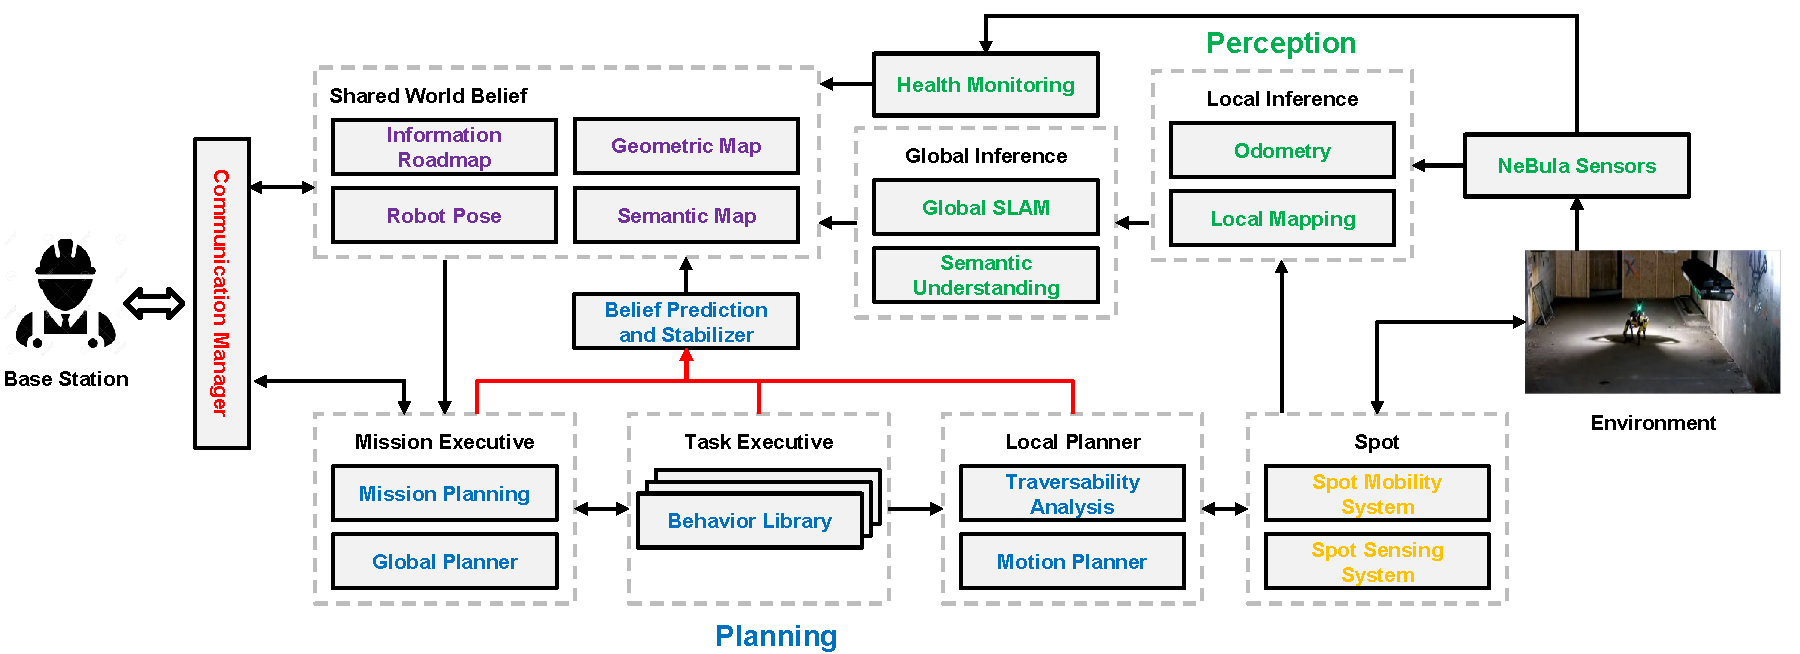
\includegraphics[width=0.9\textwidth]{graphics/spot_sa_v4.pdf}
  \caption{Overview of the system architecture \rev{that powers}NeBula and enables high-level autonomy on Spot. \rev{Red paths denote NeBula's belief-aware planning where the planner aims to minimize mission risk by steering the inference.} 
  %The red arrow highlight the belief-aware planning of NeBula where the planner try to stir the inference system to minimize mission risk.
}
  \label{fig:spot_sysarch}
\end{figure*}

\ph{Legged Mobility}
Legged robots offer unique mobility \rev{capabilities which makes them highly suitable to traverse challenging environments which would prove difficult for wheeled robots.}
%that can adapt to various challenging environments. 
They have the \rev{ability} to meet locomotion, payload, size, and endurance requirements \rev{to operate in extreme environments.} %of the \rev{DARPA}missions. 
ANYmal~\cite{whyrobotdeepmines,Bellicoso2018}, Robosimian~\cite{Karumanchi2017}, DRC-HUBO+~\cite{jung2018development}, Nimbro Momaro~\cite{schwarz2017nimbro}, MIT Cheetah~\cite{mit_cheetah}, BigDog~\cite{bigdog}, Ghost Robotics~\cite{miller2019tunnel} are just a few examples of such powerful systems. 
%However, the research community is in the just at the beginning of the road to enable these machines to autonomously carry out complex and full missions in challenging real-life environments \cite{Delmerico2019}.

\rev{The robotics research community is now in the early stages of empowering legged robots with high levels of autonomy to carry out complex missions in challenging, real-life environments~\cite{Delmerico2019}.}

\rev{Ramezani et al.~\cite{Ramezani2020}, equipped the ANYmal quadruped with a LIDAR SLAM framework for autonomous mapping capabilities. Their particular solution requires manual teleoperation to build an initial map of the environment, upon which the robot can then autonomously navigate within that map and react to previously un-mapped obstacles. 
%employ its global planner and perform autonomous exploration within the manually attained map. 
The researchers successfully demonstrated autonomous point-to-point navigation in an industrial complex.
%In \cite{Ramezani2020}, the authors first generate a global map by teleoperating an ANYmal quadruped which has been equipped with LiDAR SLAM.Subsequently, a global planner is employed to navigate the quadruped to any goal point within the constructed map, which even re-plans in the case of newly appeared obstacles.
%They successfully demonstrated autonomous point-to-point navigation in an industrial complex containing stairs.
%In \cite{Ramezani2020}, the authors describe their system which consists of an ANYmal quadruped running LiDAR SLAM. %8
%While they require teleoperation to build an initial map of the environment, from then on they can send the robot to any given goal within that map, considering terrain traversability. %4, better English, write critique more positive

Bayer et al.~\cite{Bayer2019}, demonstrate fully autonomous exploration in rough, single-level, indoor and outdoor terrains.
%in- and outdoors.
The researchers augmented an experimental hexapod platform with commercial vision sensors which they used for localization and terrain mapping.
%As experimental platform, they used a hexapod which has been equipped with commercial vision sensors for localization and terrain mapping.
%Bayer et al. \cite{Bayer2019}, demonstrate the capabilities of small hexapods equipped with low-cost commercial vision sensors, which are used for localization and mapping.
%Their hexapod is shown autonomously exploring rough terrain in-% and outdoors within a single level. %4, more positive  (p2)
%Recently, Miller et al. \cite{Miller2019} proposed the first work that goes towards full autonomy with quadrupeds in GPS-denied environments. Their Ghost Vision 60 was equipped with a high level of autonomy to explore tunnel-like environments during the DARPA Subterranean Challenge, Tunnel Circuit.
%Impressive results have been shown in  Miller et al. \cite{Miller2019}, who paved the way towards fully autonomous exploration of unknown, GPS-denied, subterranean environments with legged robots. The authors adopted a Ghost Vision 60 with a high-level of autonomy to explore tunnel-like environments during the 2019 DARPA Subterranean Challenge, Tunnel circuit.

Miller et al.~\cite{Miller2019}, 
%have demonstrated impressive results with their legged platform. They 
endowed a Ghost Vision 60 quadruped with higher levels of autonomy to explore a tunnel environment during the 2019 DARPA Subterranean Challenge, Tunnel Circuit. To our knowledge, they were one of the first researchers to demonstrate  
%paved the way towards 
autonomous legged exploration in unknown, GPS-denied, subterranean environments.} %Their solution was ideal for single-level, tunnel-focused autonomy.}

% \todo{fadil} \ph{Quadrupet real world applicationt: Anymal, Ghost, and Spot!}
% \inst{we should say great and positive things about Ghost and Anymal. and mention the state of practice in their autonomy...
% It should NOT be a "comparative paper". Instead of saying we are better, say that this is the "first autonomous behaviors in this scale on Spot". Compare the current results with the past results for Spot (rather than comparing with other platforms).}
% While various legged mobility solutions have been developed recently, 
% % Fadhil: cite 2-3 legged robot platform papers, 
% they have been minimally utilized  in  real-world  autonomous  applications\cite{whyrobotdeepmines}. 
% %
% One reported solution is an application of quadrupedal robot ANYmal in industrial inspection and search and rescue\cite{Bellicoso2018}.
% %
% In DARPA SubT Challenge, PLUTO team deployed multiple Ghost Robotics (GR) Vision 60 quadrupeds autonomously.\cite{miller2019tunnel}
% %
% While in industry world, Boston Dynamics' Spot, a direct successor to Big Dog\cite{bigdog}, shows impressive result in various applications(cite Spot web pages).
% %
% Recently, Boston Dynamic starts leasing their Spots to various industry and research communities to develop Spot application in real-world problems.

% % -Anymal: Anymal in real world application, Anymal‐toward legged robots for harsh environments. Advanced Robotics\cite{hutter2017anymal} 
% % - Ghost robotics: Upenn's Mine  Tunnel  Exploration  using  Multiple  Quadrupedal  Robots.

% % % another example
% % publicized work in 2008 . Recently they start collaborating.
% % How we expand Spot capability in extreme environment
% % emphasize our pioneer work in Spot autonomy

\ph{Contributions} %{Scope}
In this work, we focus on Boston Dynamics' Spot robot (Fig. \ref{fig:stairs-firstPage}). 
We briefly discuss the NeBula (Networked Belief-aware Perceptual Autonomy) \rev{architecture}and explain some elements of integrating full autonomy on the Spot robot.
We describe the induced behaviors and performance of the system in a complex autonomous mission \rev{during the Urban Circuit of the DARPA Subterranean Challenge.}
%\rev{in which our team took 1st place at the Urban Circuit of the}
%led to the first place at the Urban Circuit of 
%DARPA Subterranean (SubT) Challenge. 
While the main objective of this paper is to provide a system-level overview of the entire autonomy stack and robot locomotion, we will describe in further detail some specific aspects of the algorithms that are critical to enabling legged autonomy in complex missions. 
%In particular, a few highlights 

Highlights of this paper or areas where we \rev{advance}the current state-of-practice on Spot \rev{and legged robots}are:
\begin{enumerate}
    \item \rev{Endowing a legged platform with high-level autonomy so that it may traverse} %Enabling a legged platform to traverse
    distances greater than 1km in a multi-level, underground, GPS-denied environment \rev{within}
    % inless than 
    60 minutes. 
    %with high-levels of autonomy. 
    %Demonstrating he performance at the Urban Circuit of the DARPA Subterranean Challenge.
    \item Enabling reliable multi-sensor odometry in perceptually-degraded environments.
    \item Demonstrating \rev{perception- and traversaility-aware}local planning on legged platforms to negotiate challenging terrains 
    %and limited sensing capabilities.
    \rev{and perceptually-degraded environments.}
    \item Developing a robust, lightweight and rugged hardware architecture to facilitate extreme exploration and high-level sensing, communications and computational necessities.
    %\item Demonstrating real-world complexAddressing challenges in operating multi-robot simultaneously, exploring complex environments, and intermittent communication by deploying Nebula's mission planning modules
    %\item Discussing what we learned during design, testing, and operation of Nebula's powered Spot
\end{enumerate}

\rev{The performance of these technologies was successfully field-proven at the Urban Circuit of the DARPA Subterranean Challenge, where it contributed to winning first place.}

\ph{Outline}
In Section \ref{sec:nebula}, we describe the elements of the NeBula \rev{architecture}at its \rev{conceptual}layer. 
In Section \ref{sec:spot}, we discuss the \rev{legged mobility system}and the payload. Sections \ref{sec:state_estimation}, \ref{sec:local_planning}, and \ref{sec:mission_planning} focus on \rev{selected}algorithmic aspects of legged robot odometry, local planning, and high-level mission planning. 
Experimental results are presented in Section \ref{sec:experiments}, followed by future work discussion and conclusions in Section \ref{sec:conclusions}.

%%%%%%%%%%%%%%%%%%%%%%%%%%%%%%%%%%%%%%%%%%%
\section{NeBula Autonomy}\label{sec:nebula}
%%%%%%%%%%%%%%%%%%%%%%%%%%%%%%%%%%%%%%%%%%%
Motivated by autonomous exploration of extreme surfaces and subsurface terrains on the \rev{Moon, Mars}and other planetary bodies, \rev{NASA's Jet Propulsion Laboratory (NASA JPL)}is developing an autonomy architecture referred to as NeBula (Networked Belief-aware Perceptual Autonomy). 
The main focus of NeBula is to provide computationally tractable methods to predict and assess various outcomes and risks in uncertain settings. \rev{These methods subsequently}enable reliable, coordinated multi-robot exploration of unknown and hard-to-access terrains. %6.5
%To deal with unknown environments and uncertain settings, NeBula takes a probabilistic approach to model uncertainty.

\rev{To deal with uncertainty in unknown environments, NeBula employs a probabilistic approach.
%NeBula adopts a probabilistic approach to model the uncertainty. 
It fuses various sensing modalities with consideration for uncertainty-awareness. NeBula then creates a probabilistic representation of the robot's knowledge of the environment, assigns risk values to the available actions, and proactively plans to minimize the overall mission risk.} %6.5

%It and takes the uncertainty into account to probabilistically fuse various sensing modalities, creates a probabilistic representation of the robot's knowledge of the environment, computes risk, and "proactively" plans to minimize the mission risk. 

\ph{Architecture} NeBula consists of multiple components, briefly described in the rest of the paper.
Fig. \ref{fig:spot_sysarch} illustrates a high-level overview of this architecture and how its modules are interconnected. 
Spot's internal locomotion model and inbuilt factory sensors, and NeBula sensors encapsulate the overall dynamics models of the system.
%The Spot locomotion and sensing module, and NeBula sensors encapsulate the dynamics models of the system, sensors. %\st{models}
We will discuss this block further in Section \ref{sec:spot}.
The odometry module \rev{is responsible for measuring and estimating the state and relative motion of the robot.}
%contains algorithms to measure and estimate the relative motion of the robot.
We will discuss some aspects of odometry on legged systems in Section \ref{sec:state_estimation}. 
The estimated odometry is then used within the front-end of our global SLAM \rev{module}(detailed in~\cite{Ebadi2020}). 
\rev{The shared world belief block compiles the robot's model of the environment.}
The planning block, includes the 1) mission planning module that switches between various behaviors \rev{such as}exploration, stair-climbing, communication-recovery, etc., 2) global planning \rev{as well as}3) \rev{traversability analysis and motion planning.} 
\rev{The belief prediction and stabilizer module project the belief from the feedback of planning modules.}
We will discuss these modules and highlight their uncertainty- and perception-aware aspects in Sections \ref{sec:mission_planning} and \ref{sec:local_planning}. 
The communication block is responsible for enabling data exchange between the multiple robots and a base station\rev{(described in~\cite{Otsu2020})}. 

% Backup
% \ph{Architecture} NeBula consists of multiple components, briefly described in the rest of the paper.
% Fig. \ref{fig:spot_sysarch} illustrates a high-level overview of this architecture and how its modules are interconnected. 
% The locomotion/sensing module encapsulates the dynamics models of the system, sensors, %\st{models}, 
% and the API to send commands to the robot and read its sensory data. 
% We will discuss this block further in Section \ref{sec:spot}.
% The odometry block \rev{is responsible for measuring and estimating the state and relative motion of the robot.}
% %contains algorithms to measure and estimate the relative motion of the robot.
% We will discuss some aspects of this block in Section \ref{sec:state_estimation}. 
% The estimated odometry is then used within the front-end of our global SLAM \rev{module}(detailed in \cite{Ebadi2020}). The planner block, includes the 1) mission planning layer that switches between various behaviors \rev{such as}exploration, stair-climbing, communication-recovery, etc., 2) global motion planning \rev{as well as}3) \rev{traversability analysis and local motion planning.}We will discuss these modules and highlight their uncertainty- and perception-aware aspects in Sections \ref{sec:mission_planning} and \ref{sec:local_planning}. 
% The communication block is responsible for enabling data exchange between the multiple robots and a centralized server\rev{(described in \cite{Otsu2020})}. 

%%%%%%%%%%%%%%%%%%%%%%%%%%%%%%%%%%%%%%%%%%%
\section{Au-Spot Mobility System}\label{sec:spot}
%%%%%%%%%%%%%%%%%%%%%%%%%%%%%%%%%%%%%%%%%%%
\ph{Locomotion System} 
Spot is a quadrupedal robot developed by Boston Dynamics to provide mobility \rev{on challenging terrain, which cannot be accessed by traditional ground robots.
%in extreme environments and conditions. 
Spot can negotiate challenging non-planar terrain on a variety of surface types, including stair climbing.}

%Spot can traverse various terrain types, including grass, sand, and gravel at slopes of up to $\pm$30~deg. 
%It has separate gaits for dynamically stable movement, uneven terrain, and stair climbing. %Spot can carry external payloads in excess of 14~kg operates for 90~minutes  (mixed usage). 

%NeBula has the ability to autonomously command Spot's locomotion in several aspects.

% It can carry about 14 kg of payload and it lasts about 90 min. Boston Dynamics offers a wide range of low--level motion planning algorithms. The developer can use the Boston Dynamic API to access internal sensor and map data and also send velocity of waypoint commands for the internal planner.

\ph{Sensing system} 
Spot's factory perception package from Boston Dynamics comprises five custom RealSenses distributed around the \rev{robot.}Considering Spot’s overall traversability capabilities, mechanical constraints, and integration complexities, NASA JPL's NeBula Sensor Package (NSP) provides %a vehicle-agnostic and 
a parallel perception system (Fig. \ref{fig:spot_full_nebula_form}) to enable higher levels of autonomy. 
%is designed with consideration for Spot’s overall traversability capabilities, mechanical constraints, and the sensor requirements of NeBula autonomy (Fig. \ref{fig:spot_full_nebula_form}). 
The Nebula Sensor Package includes a LIDAR, Intel RealSense cameras, high-intensity LEDs, and a thermal camera.
\rev{These sensors are integrated into a shock-absorbing, rigid mechanical super structure.}Spot is a fast-moving quadruped with the ability to traverse rough terrain. 
With NeBula autonomously driving this capability to its limit, the NSP can experience significant forces, moments, and vibrations. 
A combination of hard resin urethane, semi rigid carbon-infused nylon, and aluminum are used in the manufacturing process for increased rigidity and lightweight build. 
%As Spot is being used with NeBula as a research platform while pushing the envelope of the current state of the art of autonomous systems, 
Further, the design takes into consideration atypical load paths for shock absorption during falls. %Furthermore, the  sensor package needs to be adaptable to changing requirements. This is pertinent when competing in a DARPA challenge where the understanding of the competition and environment is rapidly evolving.
%\begin{figure}[h!]
%  \centering
%  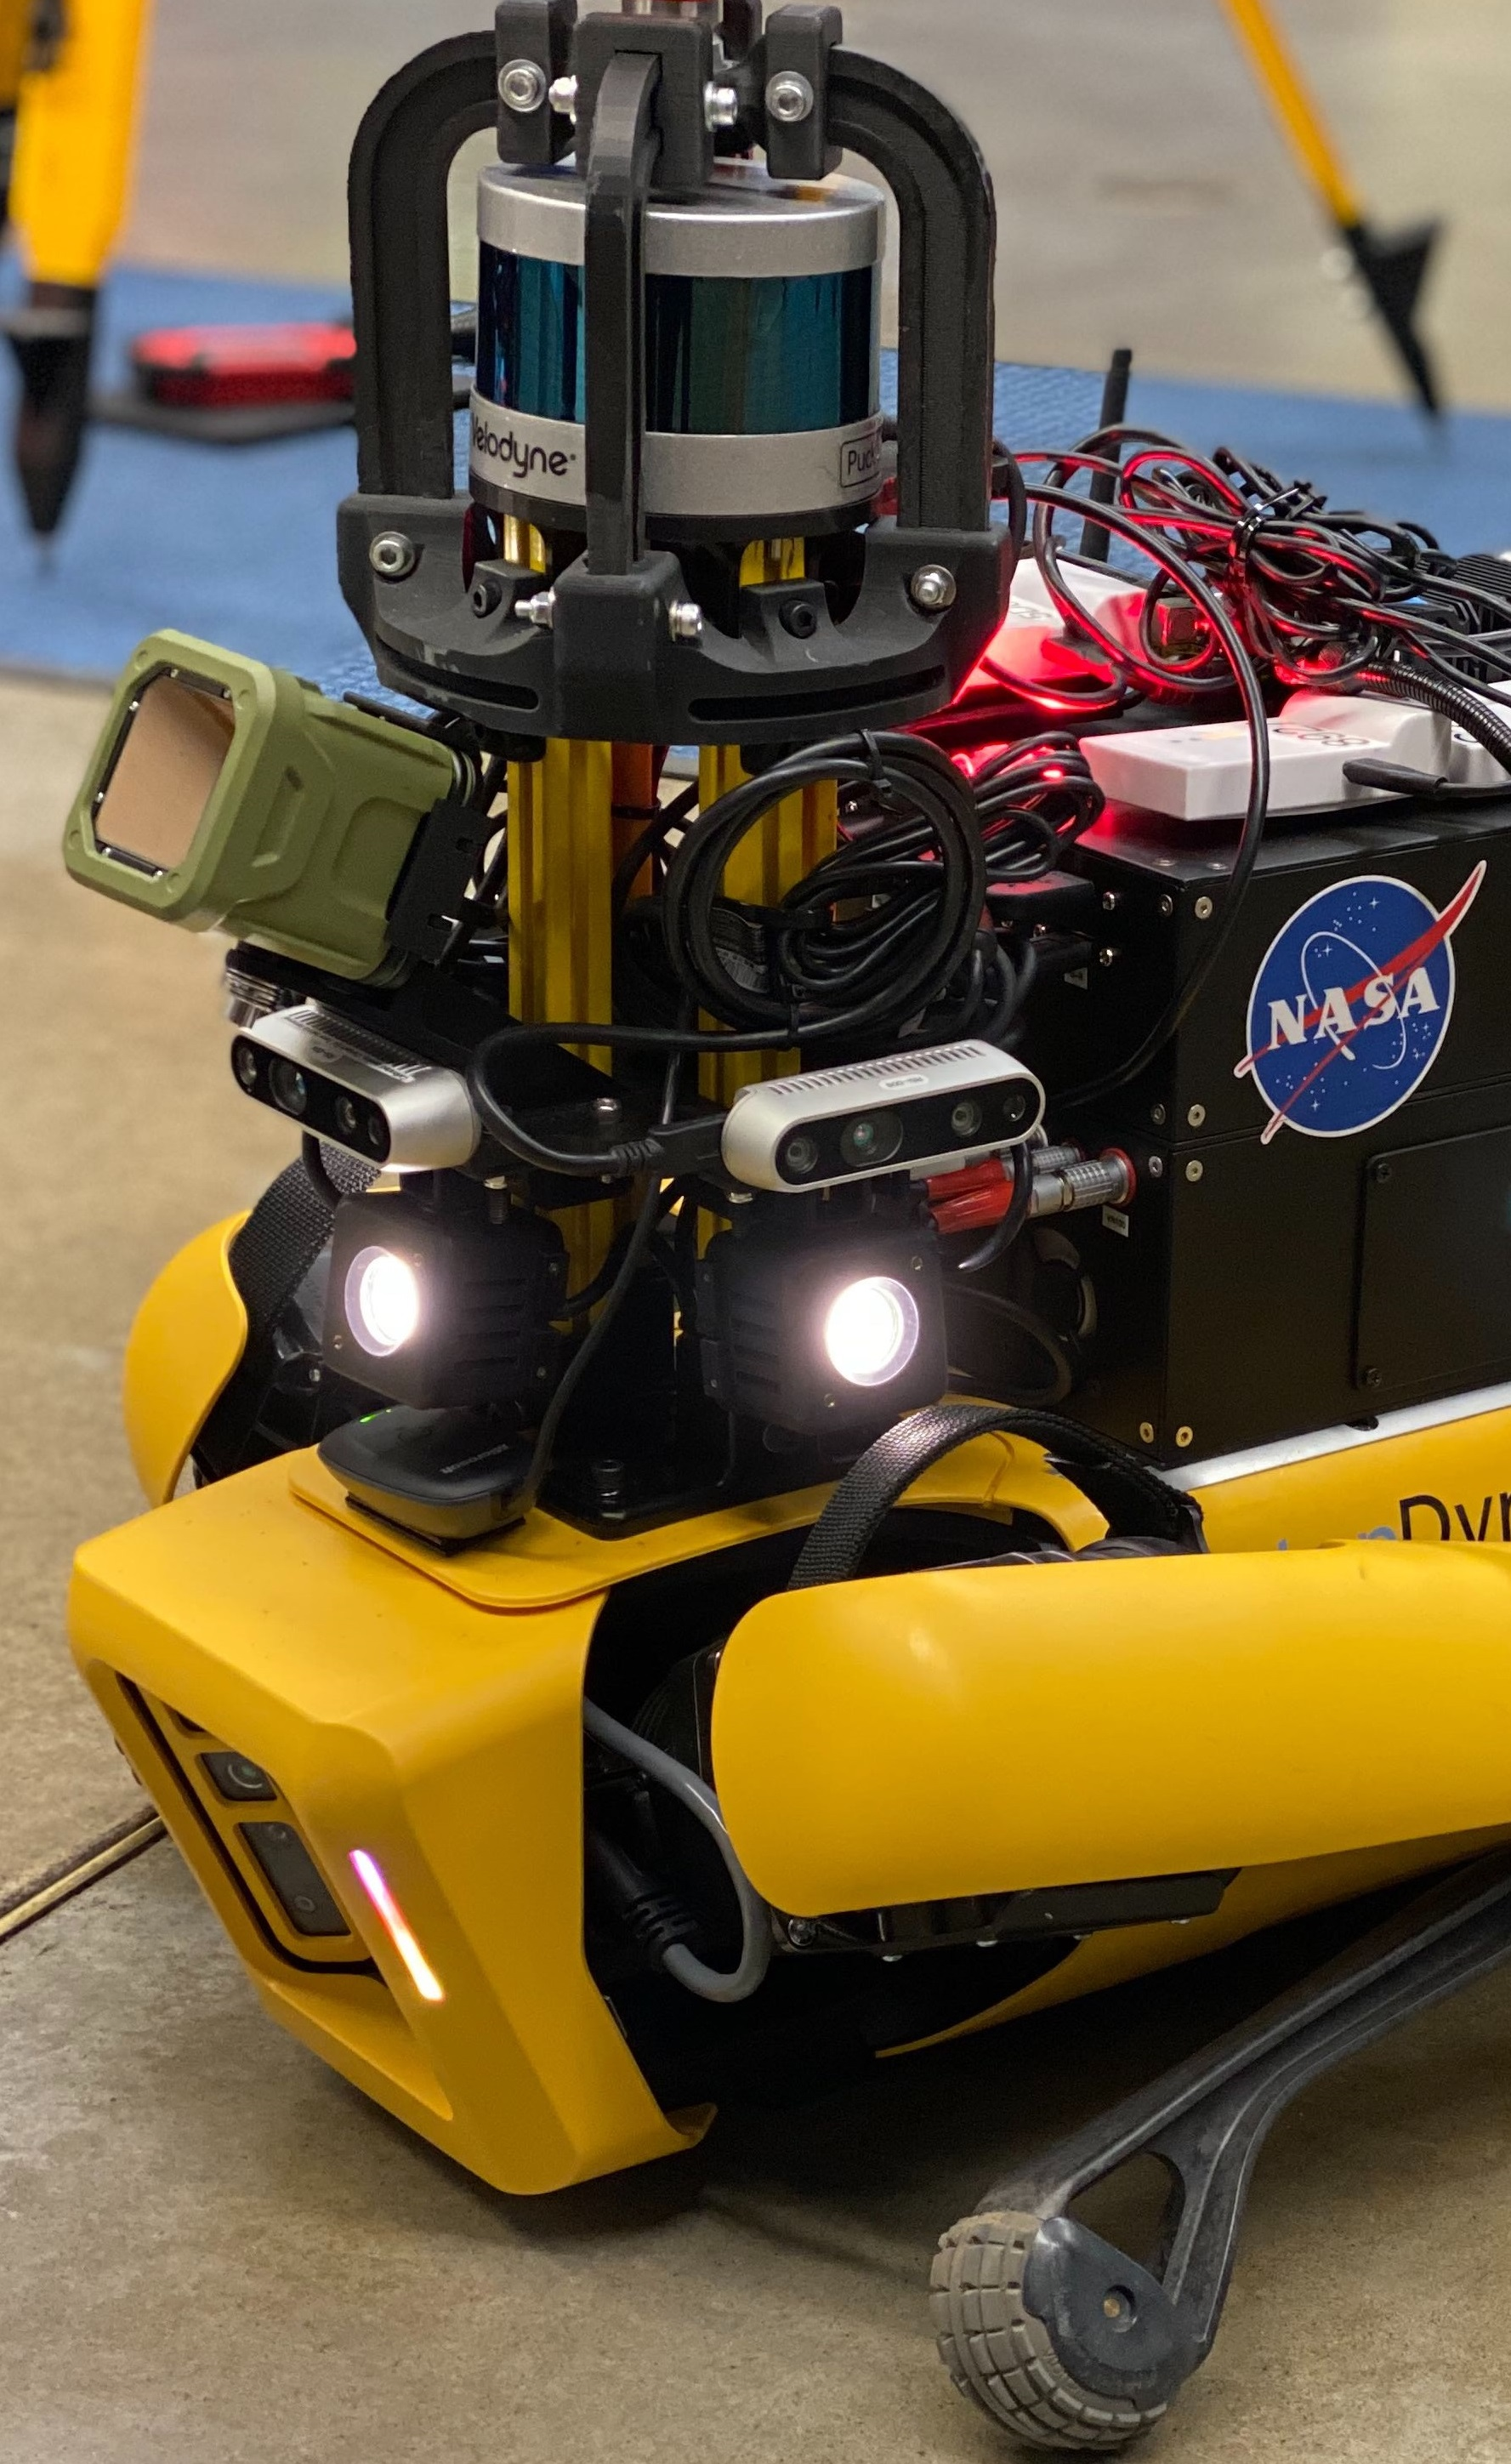
\includegraphics[width=0.2\textwidth]{graphics/spot_sensor_package_NSP_2.jpg}
%  \caption{Spot with Nebula Sensor Package Mounted}
%  \label{fig:spot_payload}
%\end{figure}
\rev{In this paper, we refer to the NeBula-powered Spot as 'Autonomous Spot' or 'Au-Spot' [/awe-spot/].} 
%(\textbf{Au}tonomous \textbf{S}ensing, \textbf{P}erception, \textbf{O}dometry and \textbf{T}raversability)


\ph{Power and Computing}
The NeBula Power and Computing Core (NPCC) is designed to mount onto Spot as an auxiliary payload which provides power to all of the NeBula sensors and the computers used for autonomy. The payload enclosure is designed with aluminum to provide protection to the internal electronics if Au-Spot were to fall. 
The payload is powered from an external lithium high capacity battery to provide isolation and extended battery life for Spot's internal battery. 
The NPCC also features a custom power distribution and safety module, which provides fuses, overcurrent protection, overvoltage protection, inrush current limiting and power sequencing of five high efficiency voltage regulators for the sensors, lights and computers. %In addition, the power module manages the physical and remote e-stops and safety systems for the vehicle. Communication to the human supervisor is achieved using a Silvus Technologies Streamcaster radio. High bandwidth communication between the computers, radio, LIDAR and Spot is done through Ethernet via an internal network switch. The cameras, IMU and UWB modules interface to the computers via USB through multiple powered hubs. 
The payload uses two high-power computers 
%(Intel and Nvidia) 
for sensing, autonomy and \rev{semantic scene}understanding.

\begin{figure}[t]
  \centering
  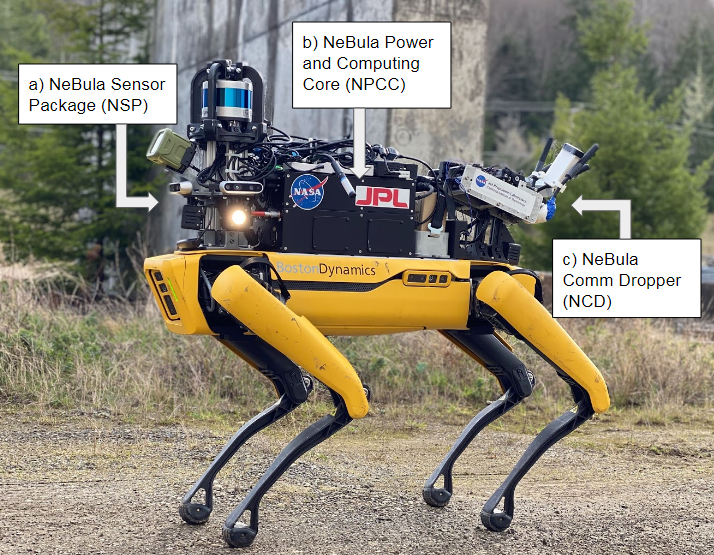
\includegraphics[width=0.45\textwidth]{graphics/spot_full_annotated_1.PNG}
  \caption{Autonomous Spot \rev{(Au-Spot)}in its 
  %in its full, 
  NeBula powered form.}
  \label{fig:spot_full_nebula_form}
\end{figure}

%\begin{figure}[thpb]
 %  \centering
  %  \begin{subfigure}[t]{0.5\linewidth}
   %     \centering
    %    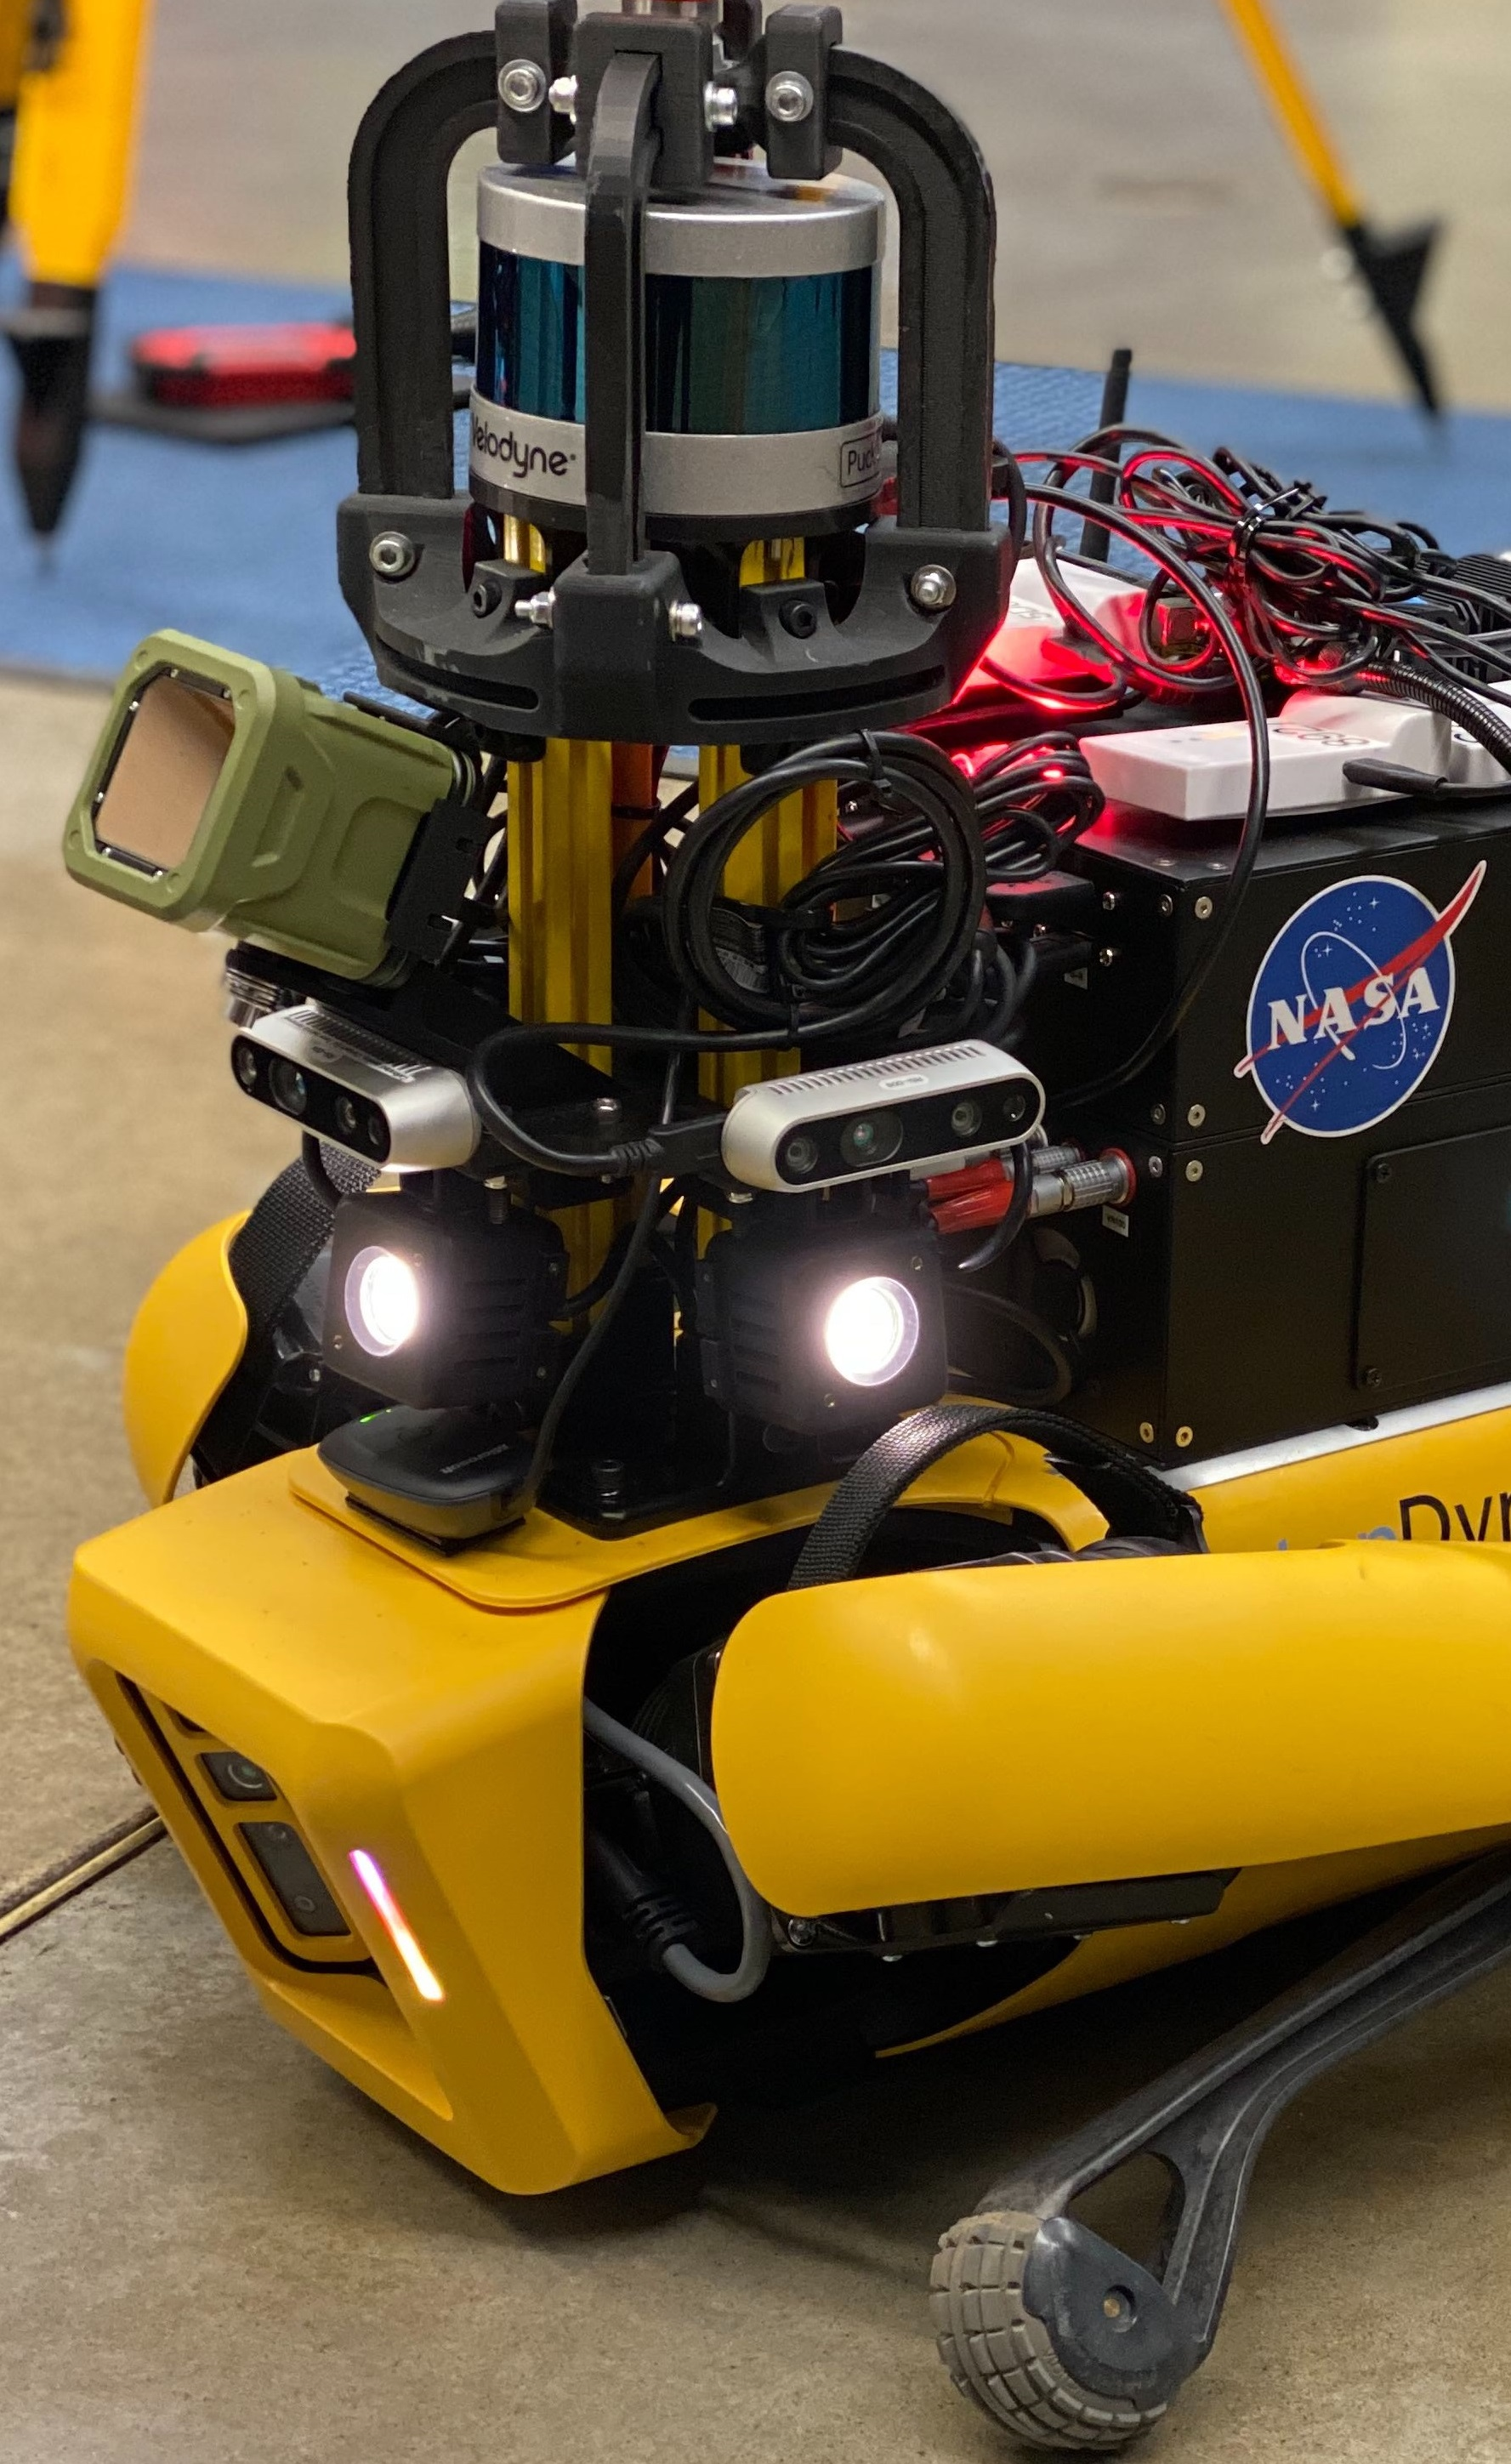
\includegraphics[width=\textwidth]{graphics/spot_sensor_package_NSP_2.jpg}
     %   \caption{Spot with Nebula Sensor Package Mounted}
      %  \label{fig:spot_payload_sens}
    %\end{subfigure}%
 %~
  %  \begin{subfigure}[t]{0.5\linewidth}
   %     \centering
    %    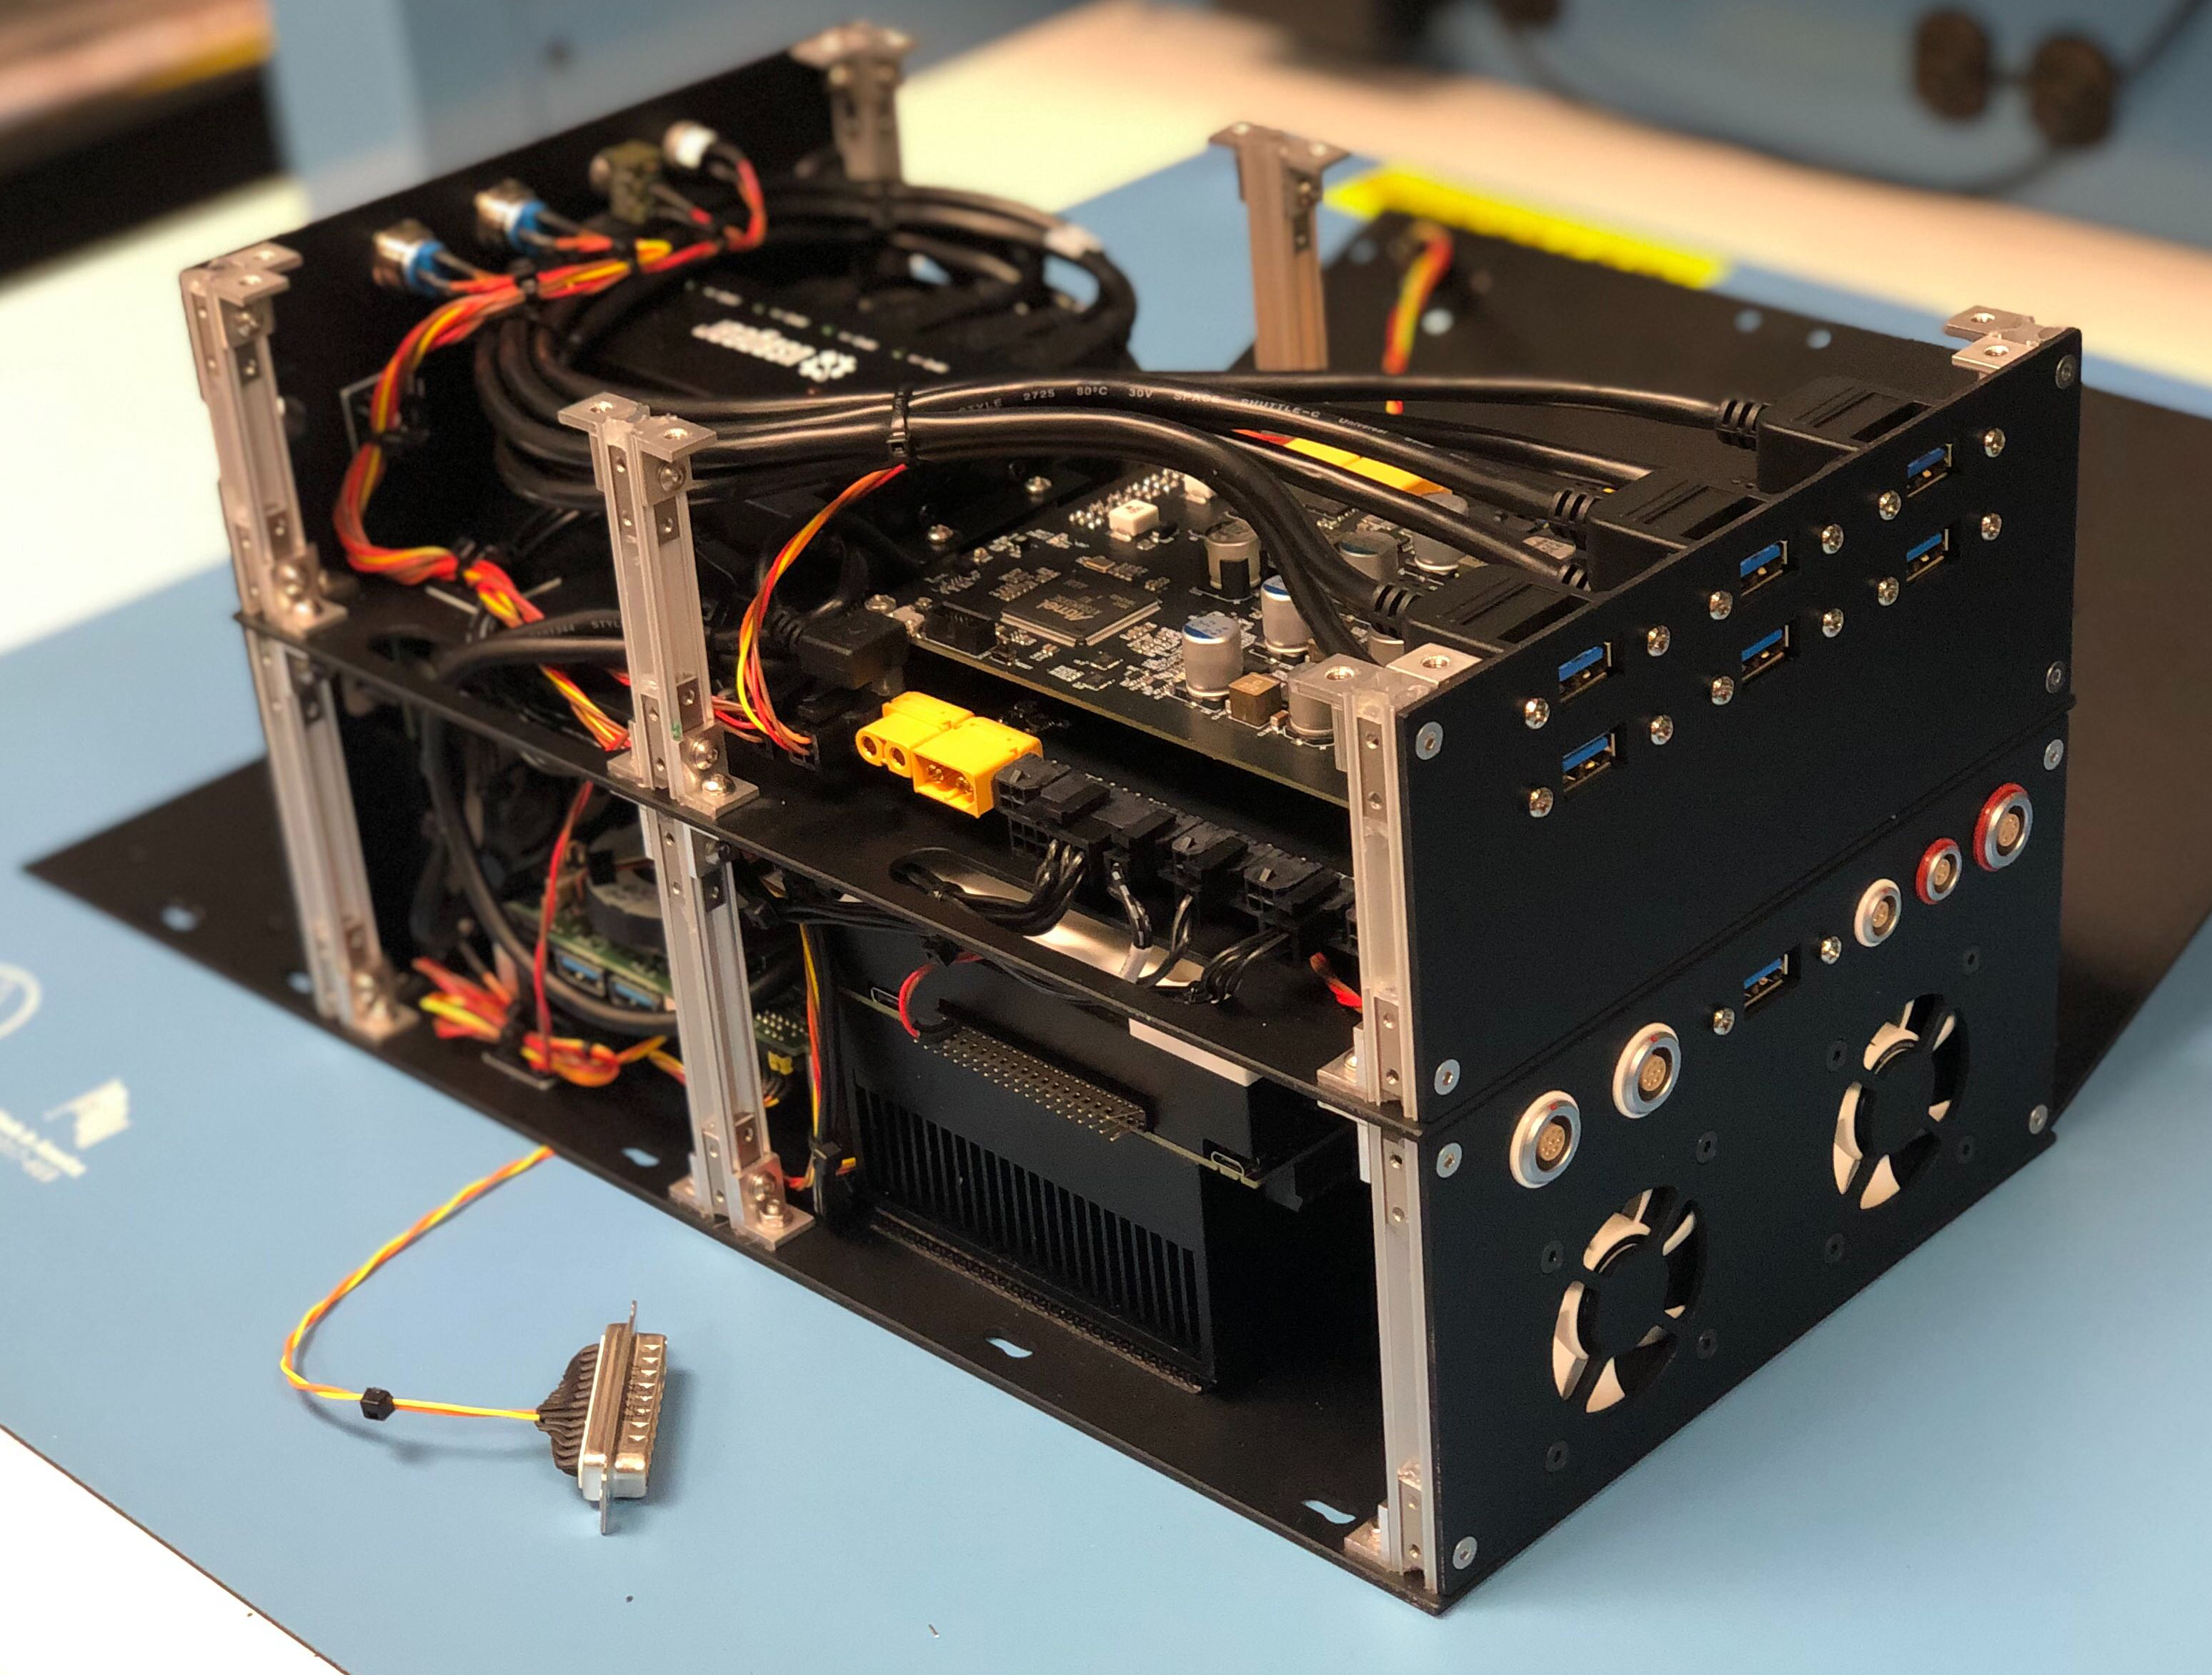
\includegraphics[width=\textwidth]{graphics/Spot_NPCC.jpg}
    %    \caption{Nebula Power and Computing Core with Covers Removed}
     %   \label{spot_payload_elec}
    %\end{subfigure}
    
%~
 %   \caption{NeBula Payload}
%\end{figure}

%\begin{figure}[h!]
%  \centering
%  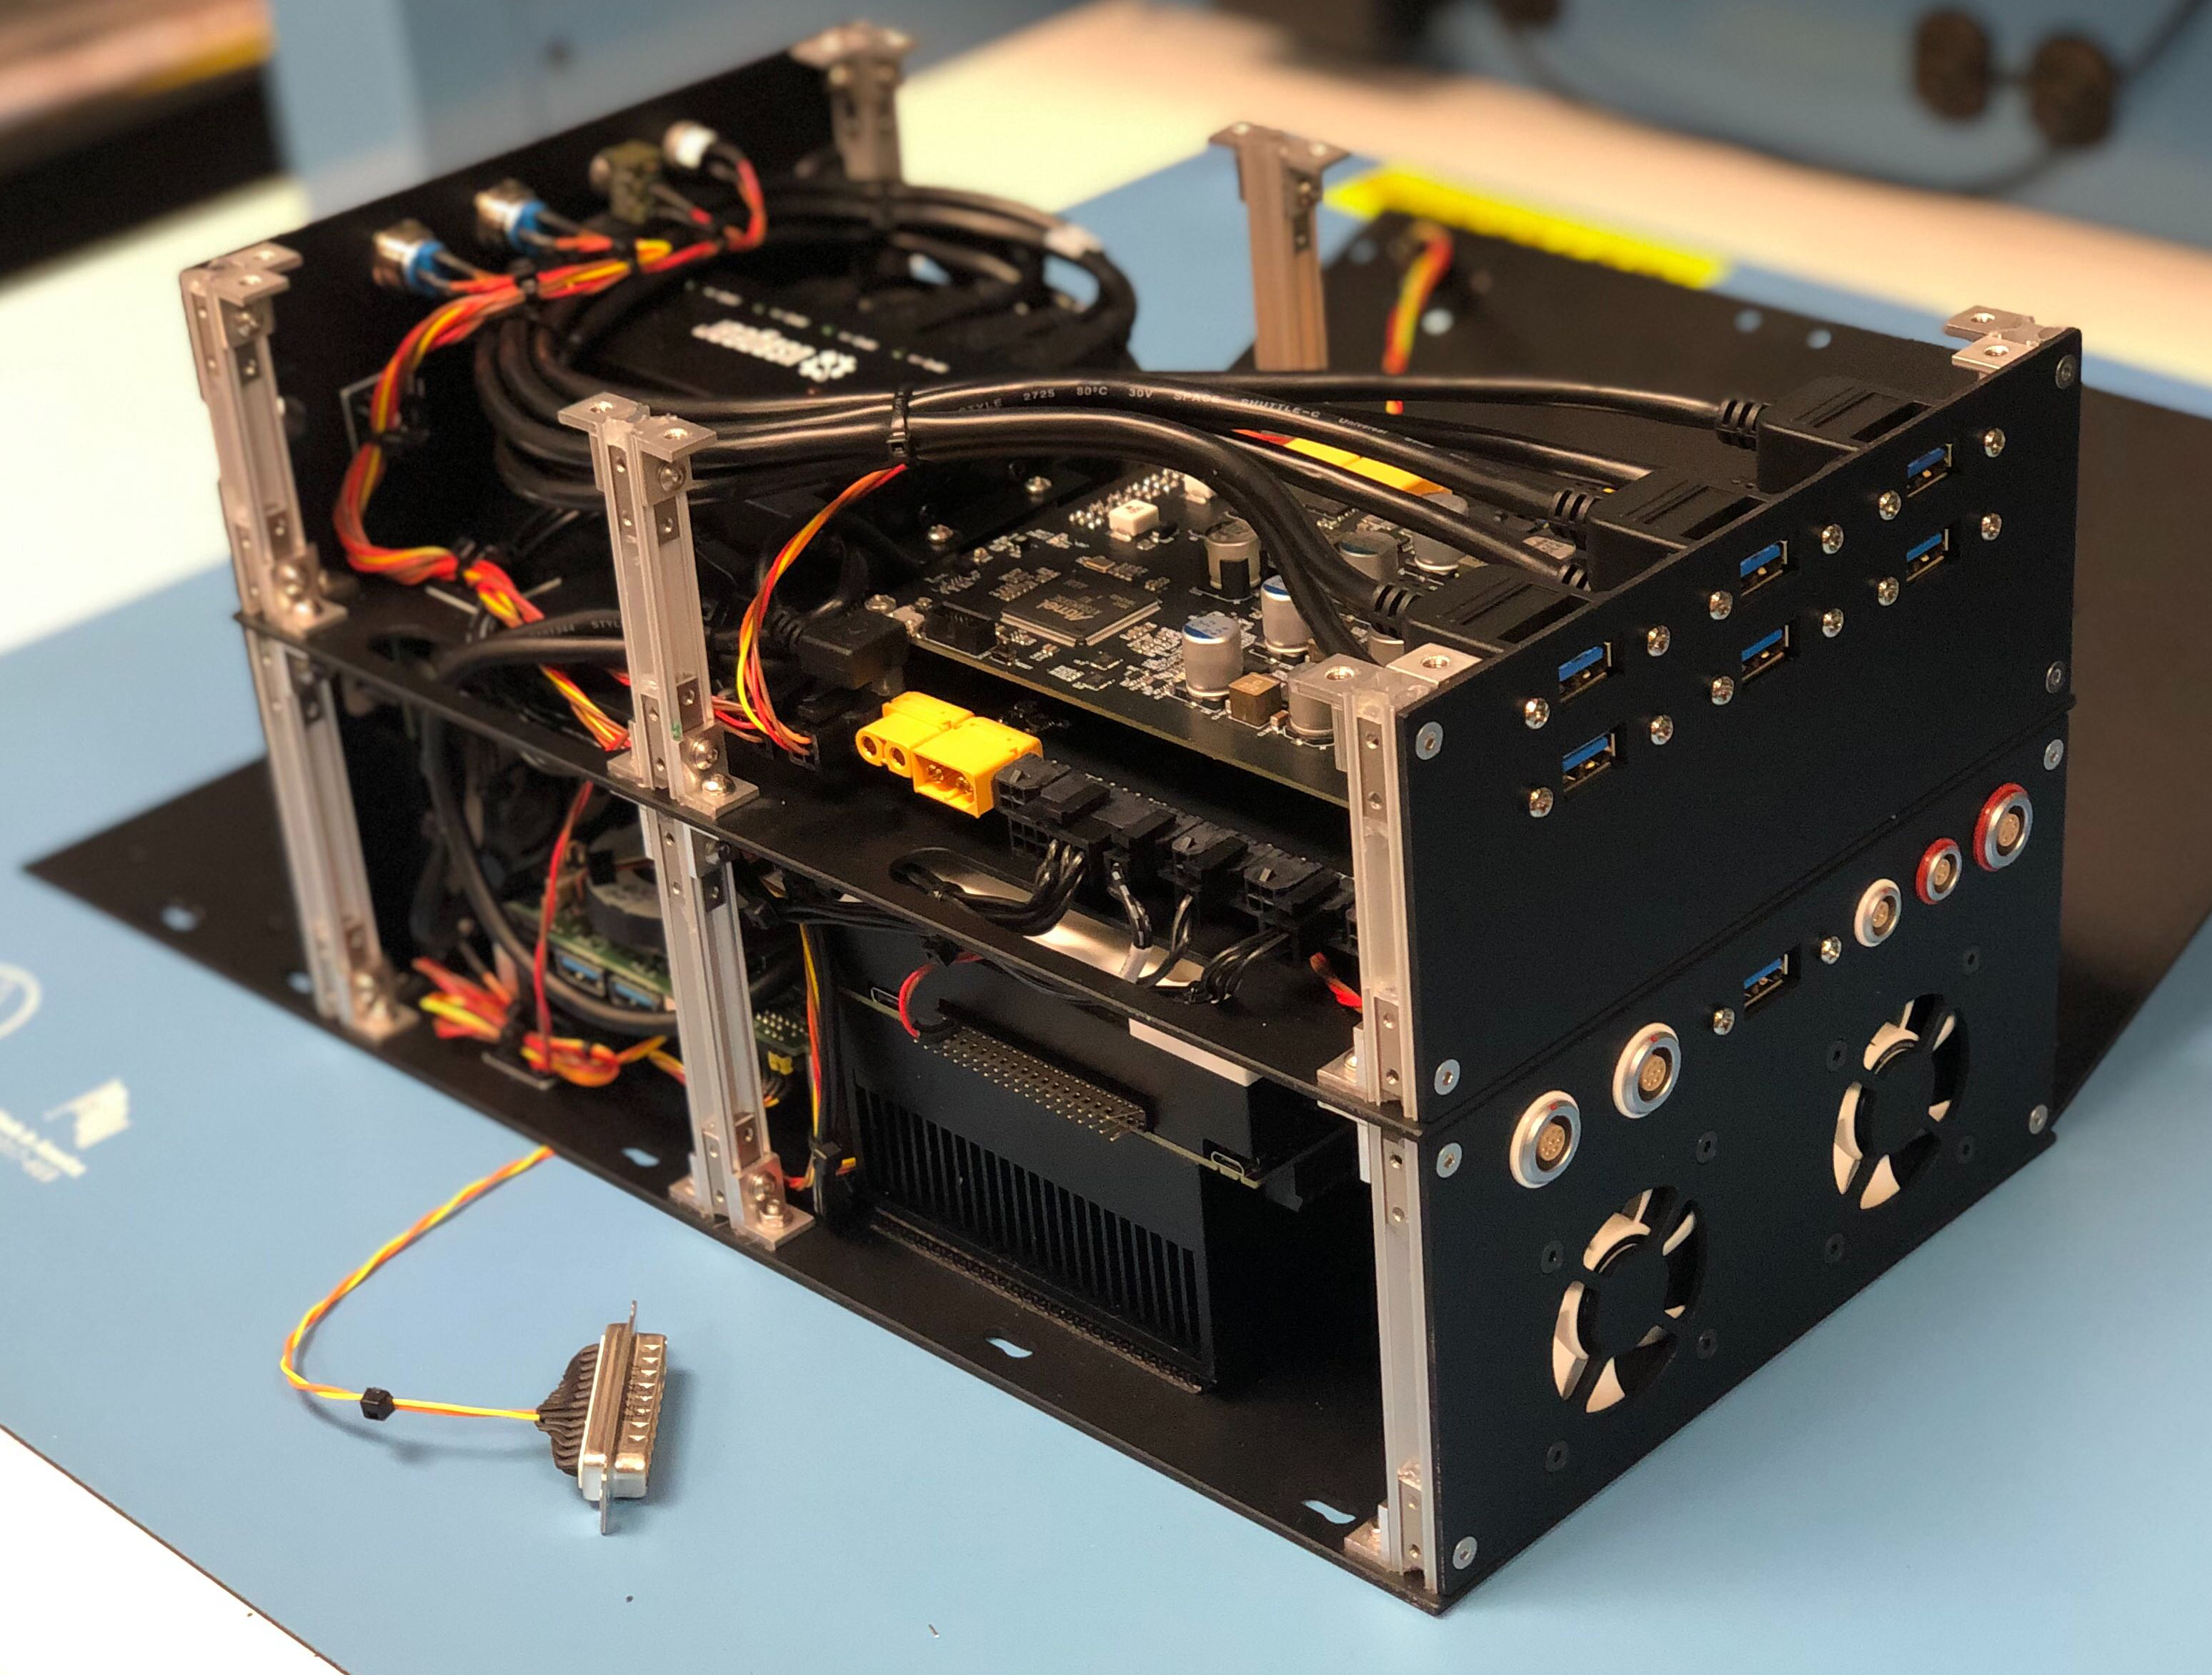
\includegraphics[width=0.3\textwidth]{graphics/Spot_NPCC.jpg}
%  \caption{Nebula Power and Computing Core with Covers Removed}
%  \label{fig:spot_payload}
%\end{figure}

% \inst{we dont need API discussion}
% \subsection{Spot Software Development API}
% \ph{Description of how program Spot through its accessible GRPC-based API and Python client library.}
% The Spot Software Development Kit enables your application to command poses and velocities, configure payloads, and access robot perception and payload data. Our Autonomy Software Development Kit, currently in Beta, will provide access to mapping, navigation, and mission editing. The API employs state-of-the-art security tools to keep your data secure.

% \ph{Robot State provided by the API and what we user}

% \ph{How to control the robot and what features are available}
% Locomotion parameter, allow obstacle avoidance, swing heights etc

% \ph{Conclude the capability of Spot and why we need NeBula to make Spot fully autonomous}

%%%%%%%%%%%%%%%%%%%%%%%%%%%%%%%%%%%%%%%%%%%%%%%%%
% \subsection{Software Interface to NeBula} % Nar5
% \inst{not very clear to me what this subsection is yet. Let's finish other parts and see if we need this}
% \ph{Overview of system integration}

% \ph{For system integration, we built the Spot driver to connect Spot API to ROS}

%\ph{Spot State}
% Robot state that we think its useful. KO, VO, Joint states, battery health

%\ph{Spot Mobility}
% Mobility setup that we think its useful: stair mode, selfright, friction coeff etc
% Stair climbing


% Spot system description will include:
% \begin{itemize}
%     \item System and locomotion system overview
%     \item Sensors description
%     \item Interfacing with Spot with API
%     \item Accessible States of the robot
%     \item Accessible locomotion, navigation feature adjustments and what we really care
%     \item Conclusion of the capability of Spot and why we need NeBula to have fully autonomous operation
% \end{itemize}









\vspace{20}

%%%%%%%%%%%%%%%%%%%%%%%%%%%%%%%%%%%%%%%%%%%
\section{NeBula Odometry on Legged Systems}\label{sec:state_estimation}
%%%%%%%%%%%%%%%%%%%%%%%%%%%%%%%%%%%%%%%%%%%



\rev{To enable autonomous robotic operation in extreme environments, a reliable odometry source is a prerequisite. In such scenarios, darkness, presence of obscurants (e.g. dust, fog, smoke), self-similar areas, along with strong platform vibration originated by mobility-stressing terrains, are common features that pose severe threats to robotic perception, making odometry estimation a challenging problem under perceptually-degraded conditions.}



\ph {Odometry Challenges} 
Uneven and slippery areas make inertial sensing inaccurate while the material composition of the surface where the legged robot is walking on (e.g soft moquette, hard concrete) has strong impacts on the accuracy of kinematic-based odometry (KO). Darkness, or sudden excessive change in illumination, along with dust and the occasional presence of fog and gas, pose significant challenges to cameras, and potential visual aliasing phenomena in texture-less or texture-repetitive environments make feature-tracking problematic, decreasing the overall reliability of vision-based odometry (VO). Self-similar environments with repetitive geometry and lack of distinctive landmarks, make scan-matching based methods ambiguous and prone to drift: moreover, active stereo cameras (including the in-built factory ones on the Spot platform) have a limited field of view and their high noise in long-range sensing render them inaccurate for this purpose.



\rev{\ph{Solution Architecture} To overcome these challenges, NeBula relies on a LiDAR-centric uncertainty-aware multi-sensor fusion framework where a \emph{selected} odometry source is fused with LiDAR information to enable accurate ego-motion estimation under challenging perceptual conditions. The main components of the proposed approach are as follows: \texit{(i)} an anomaly-aware odometry multiplexer (HeRO), \texit{(ii)} a multi-sensor LiDAR-centric SLAM front-end (LOCUS) and \texit{(ii)} a SLAM back-end (LAMP). We report in Fig.\ref{architecture} a high-level overview of the proposed approach, and discuss each sub-component in the following.} 



\begin{figure}[thpb]
  \centering
  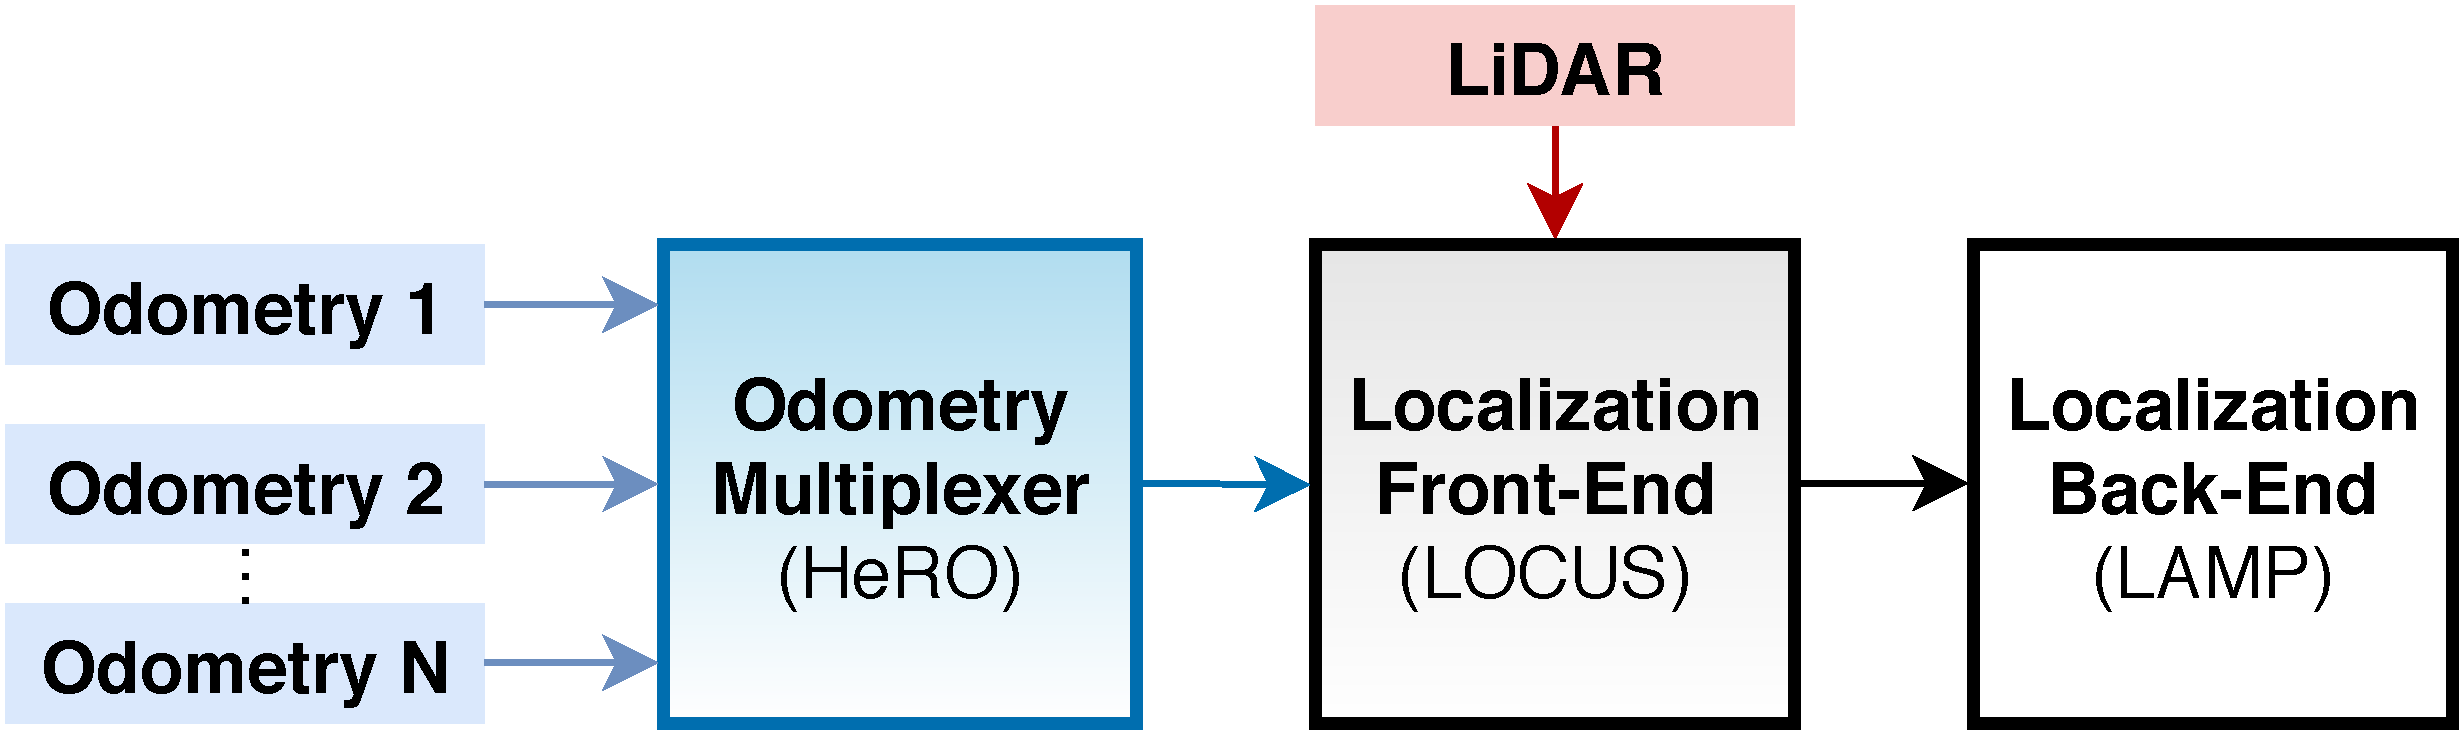
\includegraphics[width=0.49\textwidth]{spot_iros/graphics/architecture.pdf}
  \caption{\rev{Solution Architecture of the NeBula Multi-sensor Fusion Framework}}
  \label{architecture}
\end{figure}



\rev{\ph{Odometry Multiplexer} To select the best odometry source to be fused with LiDAR information, we feed multiple and heterogeneous sources of odometry available onboard (e.g. KO, VO, etc...) into an anomaly-aware odometry multiplexer, referred to as HeRO~\cite{Santamaria-navarro2019}. At every time step, HeRO runs a confidence test on each odometry source to detect potential anomalies in the estimation stream (e.g. gaps, jumps, divergences) and identify the most reliable input from a predefined ranking following a resilient paradigm: if an anomaly is detected in the highest-ranking source, then the next source in the ranking that passed the confidence check is selected. %Being $\mathcal{R}$ the coordinate system of the robot and $\mathcal{W}$ the coordinate system of the world, 
In the following we indicate the pose estimate of HeRO's output with $\textbf{Y} \in SE(3)$.
}



\rev{\ph{Localization Front-End} The output of the odometry multiplexer is fed into a multi-sensor LiDAR-centric SLAM front-end module, referred to as LOCUS~\cite{Palieri2020} that performs a cascaded GICP-based scan-to-scan and scan-to-submap matching operation to estimate the relative motion of the robot between consecutive LiDAR acquisitions. We denote with $L_{k}$ the lidar scan collected at time $k$ and with $L_{k-1}$ the lidar scan collected at time $k-1$. We indicate with $\textbf{E}^{k-1}_{k} = \textbf{Y}^{-1}_{k-1}\textbf{Y}_k\in SE(3)$ the rigid body transformation of HeRO's output between two consecutive LiDAR acquisitions. %(in order to address asynchronous odometry measurements, we interpolate the buffered $\textbf{Y}$ at LiDAR timestamps to $t_{k-1}$, and $t_k$ to get $\textbf{Y}_{k-1}$ and $\textbf{Y}_{k}$: the pose of HeRO's output at times $t_{k-1}$ and $t_k$, respectively). 

In the scan-to-scan matching stage, GICP computes the optimal transformation $\hat{\textbf{T}}^{k-1}_{k}$ that minimizes the residual error $\mathcal{E}$ between corresponding points in $L_{k-1}$ and $L_{k}$. 
\begin{align}\label{eq:GICP_ss}
\hat{\textbf{T}}^{k-1}_{k} = \arg\min_{\textbf{T}^{k-1}_{k}} \mathcal{E} (\textbf{T}^{k-1}_{k}L_{k}, L_{k-1})
\end{align}
To enhance accuracy and reduce computation we initialize GICP with $\textbf{T}^{k-1}_{k} = \textbf{E}^{k-1}_{k}$. In the case where no input is received by HeRO, GICP is initialized with the identity pose and the system reverts to pure lidar odometry. 

To enable global consistency across the history of scans, the motion estimated in the scan-to-scan matching stage is further refined by a scan-to-submap matching step. Here $L_k$ is matched against a local submap $S_k$ which is taken from the local region of the global map $M_k$ given the current estimate of the robot pose in the world frame (the global map is an accumulation of point clouds after every $t$~meters of translation, or $r$~degrees of rotation and is stored in an octree format: in our results, we use $t = 1$, $r = 30^o$).
\begin{align}\label{eq:GICP_map}
\tilde{\textbf{T}}^{k-1}_{k} = \arg\min_{\textbf{T}^{k-1}_{k}} \mathcal{E} (\textbf{T}^{k-1}_{k}L_{k}, S_{k})
\end{align}
In this optimization, $\textbf{T}^{k-1}_{k}$ is initialized with the $\hat{\textbf{T}}^{k-1}_{k}$ result from Eqn.~\ref{eq:GICP_ss}. 

After scan-to-scan and scan-to-submap matching, the final estimated motion $\tilde{\textbf{T}}^{k-1}_{k}$ between consecutive LiDAR acquisitions is used to update the robot pose in the world: the generated odometry is therefore the integration of all computed incremental transforms. 
% Both accuracy and computational speed are improved by the cascaded optimization approach: a good initial estimate in both (3) and (4) reduces the chances of converging in a sub-optimal local minima, and reduces the number of iterations needed to converge, lowering computation time.

%The key idea is to use the incremental transformations $\Delta T_{k} = T_kT^{-1}_{k-1}$ coming from the external odometry source to seed the Generalized Iterative Closest Point (GICP) algorithm in the scan-to-scan registration stage. More specifically, we initialize GICP between the Lidar scan $L_k$ collected at the current time $k$ and the LiDAR scan $L_{k-1}$ collected at $(k-1)$-th time step with the rigid body transformation resulting from the external odometry between time steps $k-1$ and $k$, namely $\Delta T_{k}$ . We then use this accurate external odometry incremental transform as the initial guess for GICP, which computes the optimal transformation $T'_{k} $ that minimizes the distance $d$ between the scan $L_{k-1}$ and the scan $L_k$ transformed by $\Delta T_{k}$. %To further enhance the accuracy of the scan-to-scan estimate, we also use a scan-to-submap matching refinement step, where the latest scan $L_k$ is matched against a local submap $M_k$.

}



\rev{\ph{Localization Back-End} The odometry produced by the front-end is fed into the back-end of our SLAM system, referred to as LAMP~\cite{Ebadi2020} which receives pose-to-pose constraints and solves a Pose Graph Optimization (PGO) and Incremental Consistency Measurement (ICM) problem for global localization when loop closures are detected during traverse.}



%%%%%%%%%%%%%%%%%%%%%%%%%%%%%%%%%%%%%%%%%%%
\section{Local Planning}\label{sec:local_planning}
%This section describes our approach to build a bigger environment map and it's use for local planning.

Assessing the traversability risk is a prerequisite for autonomous navigation in extreme environments.

%\rev{In order to accomplish the overall mission, we develop the local planner is to choose actions that minimize the failure risk to the robot.}

%\rev{In order to \rev{accomplish}the overall mission, the robot must negotiate its local surroundings and safely navigate to local waypoints. %6
%While time or distance minimization are common objectives for a local planner, we put a significantly higher emphasis on the robot's safety.
%As we are operating in unknown and challenging environments, the main objective of the local planner is to choose actions that minimize the failure risk to the robot.}

%To this end, we adopt a risk-aware local planning approach, where we analyze the traversal risk of the local surrounding and plan minimum-risk paths to a given waypoint.

%%%%%%%%%%%%%%%%%%%%%%%%%%%%%%%%%%%%%%%%%
\subsection{Traversability Map}

\rev{The traversability challenges in our mission of interest include}

%In our \rev{mission of interest,}traversability challenges include 
high slopes, obstacles, holes, deployed communication nodes, other robots, and sensor blind spots.  

In order to find a balance between efficient traversal and low risk to the platform, we construct a measure of accumulative risk for a given path through the environment.  
Let $g=(m^1,\cdots,m^n)$ be a \rev{robot-centric}grid of $n=n_l\times n_w$ cells with length $n_l$ and width $n_w$, and let each $m^i\in[0,1]$ represent the probability that the robot safely traverses through cell $i$. 
Let $\pi=\{i_t\}_{t=0}^T$ denote a path defined as a sequence of connected cells $i^t \in g$. \rev{The set of all paths that connect the current robot pose with the goal is denoted by $\Pi$.}
%Let $\Pi$ denote a set of paths that connect the current robot pose with the goal. 
%\rev{Furthermore, we define \emph{risk} as the complement of traversability $r^i = 1 - m^i$.}

\ph{Path Risk}
We define the total accumulated risk of the path $\pi\in\Pi$ as 
\begin{align}
 \mathcal{R}^{\pi}=1-\prod_{t=0}^Tm^{i_t}
\end{align}
which is the probability that the robot fails to safely traverse the path $\pi$.  

\ph{Risk Sources}
There is a variety of risk sources which can increase the probability of failure during traversal.
The most impactful sources, which are therefore considered in our analysis, include a) positive obstacles, b) negative obstacles, c) slopes, d) steps, e) mission items (other robots, deployed communication nodes), and f) sensor blind spots.

% We combine multiple layers of grids that encode different types of risk. Assuming mutual exclusivity between each risk type, the total risk in each grid cell is simply the product of the individual risks of each layer.  We consider the following sources of risk:
% \begin{itemize}
%     \item Obstacles (Walls, Rubble, etc.)
%     \item Steep Slopes
%     \item Negative Obstacles
%     \item Sensor Blind Spots
%     \item Mission Items (comm nodes, other robots, etc.)
% \end{itemize}

\rev{\ph{Multi-Range Terrain Map}}
% To identify these sources of risk, we perform traversability analysis on a local, robot-centric terrain map.
% In order to trade-off \emph{range}, \emph{coverage} and \emph{accuracy}, we construct a multi-range/multi-fidelity terrain map.
% \ph{Short range}
% On the short range ($<$ 1m), we mainly rely on the height-map created by Spot's internal depth cameras.
% For the medium range (5mx5m), we use instantaneous LIDAR point clouds.
% For the long-range (20mx20m), we build a spatial map \cite{oleynikova2017voxblox} by integrating LIDAR point clouds with odometry.
% On the short range, a step filter is applied to mark points whose distance from the local ground plane is above or below the  robot's ground clearance.
% \ph{Mid-long-range}
% On the medium and long range, we perform ground segmentation \cite{himmelsbach2010fast} and settling-based collision and stability check  \cite{krusi2017driving}.
% Settling is performed by fitting local ground planes in the point cloud terrain map. Additionally, gaps in the medium-range map are marked as negative obstacles.
% $g = \{g^{1},...g^{n}\}$
% Each risk source a.) - f.) is stored in its own risk submap $\{g_{a},...g_f\}$. 
% The maps are resolved at 2cm/cell for the medium range and 5cm/cell for the long-range.
% Deployed nodes are hazards with known locations. Blind spots correspond to chunks of unknown space in the short-range terrain map.
For detecting the aforementioned risk sources, we must build a terrain map of the robot's surrounding.
%As we are operating in unknown environments, we do not have access to prior maps.

\rev{Given that the environment is completely unknown prior to exploration, we do not have any maps, and thus}we employ the heterogeneous NeBula Sensor Package (NSP) for modeling the terrain up to 10m away from the robot.
Specifically, depth cameras are used for short range sensing ($\leq$1m), instantaneous LIDAR point clouds for medium range sensing ($\leq$3m), and spatially fused point clouds \cite{oleynikova2017voxblox} for long range detection ($\leq$10m).

\rev{The combination of these various sensing capacities yields an optimal}trade-off between \emph{range}, \emph{density} and \emph{accuracy} in the resulting terrain map.

\rev{\ph{Traversability Analysis}}
%Different sources of risk have to be detected by different methods. In addition to that, the heterogeneity of the terrain map requires us to use different methods for the \emph{same} risk type.

The listed risk sources were located by performing traversability analysis on the terrain map.
To detect positive and negative obstacles, a step filter was applied to the dense, short range terrain map. 
%A step filter was applied to the dense short range terrain map to detect positive and negative obstacles.
On the sparser medium and long range map, ground segmentation \cite{himmelsbach2010fast} and settling-based collision and stability checks \cite{krusi2017driving} were applied to detect positive obstacles and high slope regions.
In the medium range map, gaps were identified as negative obstacles.
The remaining two risk sources, deployed communication nodes and other robots, did not need a special analysis as their locations are already known.


\rev{\ph{Multi-Layer/Multi-Range Traversability Map}}
To best capture the heterogeneity across risk sources and range, we represent the traversability map in the layered architecture shown in Fig. \ref{fig:layered_costmap}.
The traversability map $g$ implicitly consists of $N$ different layers $\{g_1,...,g_N\}$. The vertical dimension separates the traversability map by risk source and the horizontal dimension separates it by the sensor used
%hence the range.
This architecture is henceforth referred to as the \emph{risk-range volume}; inspired by the  
%We will refer to this architecture as the \emph{risk-range volume}, inspired by the 
\emph{scale-space} architecture known within the computer vision community.

The process by which individual layers feed into the overall traversability map $g$, is elaborated upon below.
%How the individual layers feed into the overall traversability map $g$ is elaborated further below.

\begin{figure}[thpb]
  \centering
  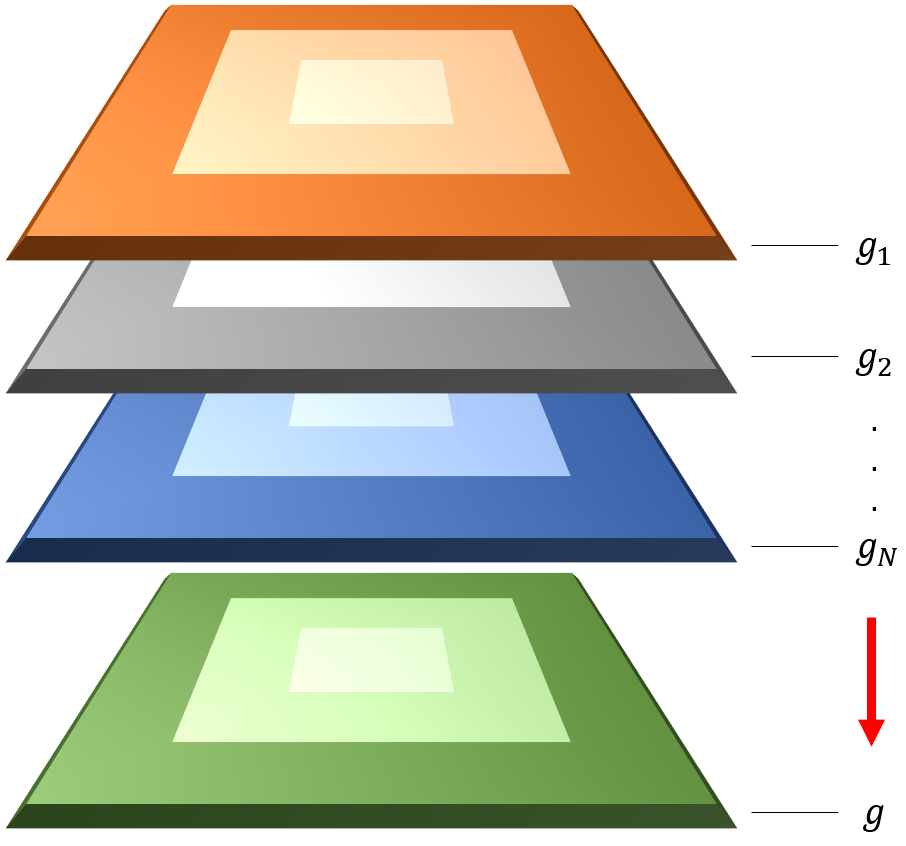
\includegraphics[width=0.35\textwidth]{spot_iros/graphics/layered_costmap.png}
  \caption{The mulit-layer/multi-range traversability map, called \emph{risk-range volume.}}
  \label{fig:layered_costmap}
\end{figure}

\ph{Sparse Traversability Evaluation}
To enable a computationally tractable traversabilty analysis in order to subsequently create the risk-range volume, we only perform traversability analysis on a representative set of query points.
The result is a sparse grid within the risk-range volume, for which the exact traversability risks are computed.

% Because of computational constraints, traversability can not be assessed for every grid cell of the map.
% Instead, traversability is only checked for a sparse set of query points.
%Hard thresholds are used for the sources a.) - c.) in order to assign binary risk values $r \in \{0,1\}$. 

\ph{Dense Approximation}
When planning smooth paths, high resolution
%it is desirable to have a high resolution 
in the \emph{range} dimension of the risk-range volume, is desirable.
We approximate the risk-range volume at a higher resolution by inflating each query point along the \emph{range} dimension.
The amount of inflation is determined by the risk value of the query point.
%A decaying inflation layer is added to any lethal point ($r=1$), which results in smooth risk maps.

% Sensor blind spots contribute a non-lethal risk and are identified by the respective sensor models.  
%Deployed communication nodes, other robots and sensor blind spots are added as blobs of high risk to their respective risk maps $g_e$ and $g_f$.

%\ph{Combined Risk}
\ph{Superposition}
%So far, t
There are \rev{$N$}different \rev{layers} $\{g_1,...,g_N\}$ for the aforementioned risk sources.
With consideration for planning purposes,
%For planning purposes, 
a single traversability map $g$ is created from the different layers.
The different risk sources are not probabilistically independent. 
\rev{However, we treat them as independent in order to approximate a conservative risk estimate by element-wise multiplication:}
\begin{align}
r^i = (1-m^i) = \prod_{k=1}^N(1-m_k^{i})
\end{align}
%The multiplication of the individual risk values does not imply probabilistic independence, but rather gives us a conservative estimate for the combined risk.

An mission obtained traversability map $g$ is shown in Fig. \ref{global_costmap}. % 4
Magenta regions indicate \emph{high} regions, cyan indicates \emph{medium} risk and dark indicates \emph{low} risk regions.

\begin{figure}[thpb]
   \centering
    \begin{subfigure}{0.49\linewidth}
        \centering
        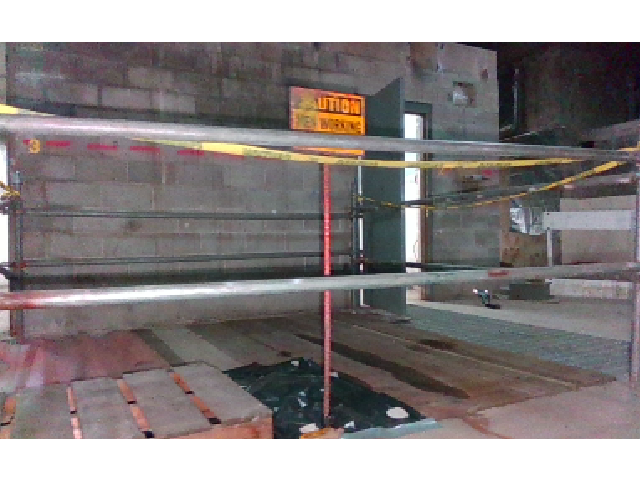
\includegraphics[trim={1cm 1cm 0cm 1cm},clip, width=\linewidth]{graphics/costmap_image.png}
    \end{subfigure}%
    ~ 
    \begin{subfigure}{0.49\linewidth}
        \centering
        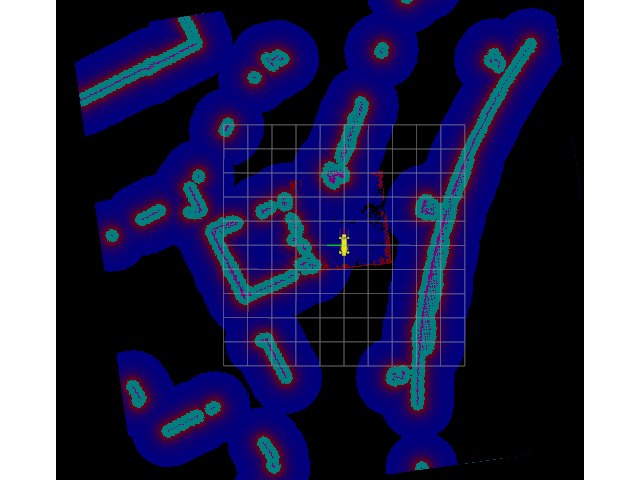
\includegraphics[trim={1cm 1cm 1cm 2cm},clip,width=\linewidth]{graphics/costmap_large.png}
    \end{subfigure}
    \caption{Left: Left camera image of a high-risk traversable region.  Right:  Risk map with obstacles in image to the left of the robot (centered); 1m markings are in gray.}
    \label{global_costmap}
\end{figure}


%Accurate risk assessment is contingent upon good localization/odometry.  When odometry fails we want our assessment of risk to remain conservative in such a way as to keep the vehicle safe at all times.  Therefore we rely on a multi-resolution approach for assessing risk.  We asses risk on a local scale (2m radius) by relying on wide-field of view sensor data with a short temporal window.  This approach relies on a short history of KO/VO odometry, which tends to have low drift at these timescales.  For areas outside this small radius (2m-10m), we rely on temporally fused sensor data using our LiDAR payload, since this sensor has much longer range and higher accuracy at these scales.  We combine these two layers to achieve both long-range mapping for efficient planning, along with high-fidelity mapping at short ranges to ensure the safety of the platform.
%\ph{Solver}

%%%%%%%%%%%%%%%%%%%%%%%%%%%%%%%%%%%%%%%%%
\subsection{Risk-Aware and Perception-Aware Planning} 
Based on the traversablility map $g$, introduced in the previous section, we formulate the risk-aware planning problem
as the process of finding a path which minimizes the overall path risk. %5
$\pi^* = \arg\min_{\pi\in\Pi}\mathcal{R}^{\pi}(g)$.
%We search for the minimum risk path using A*.
%The grid representation of the traversabiltiy map allows us to search for such a path using \rev{graph-search}algorithms,  such as A*.
%\rev{A waypoint is selected along the path and is sent to Au-Spot's proprietary planner for execution.}
%Having found the minimum risk path on the risk map, we then send a carrot waypoint 1m along this path to Spot's internal trajectory planner. 
%The proprietary planner keeps it's own small 5mx5m costmap, which is created from the platform's built-in depth cameras.
%Spot then executes the planned trajectory through its low-level controllers.
%\ph{Stair Climbing}
%A special case that is not handled by the local planner is stair climbing. \rev{Stairs will either appear as positive or negative obstacles in the risk map.} In the current setting, stair climbing is semi-autonomous. The human supervisor has to \rev {: \textit(i)} detect the presence of a stair case \rev{(e.g. from the robot Camera/LiDAR feed)}, \rev {\textit(ii)} switch Spot's internal planner to 'Stair' mode which configures the planner for climbing stairs, and then \rev {\textit(iii)} give \rev{a goal} at the end of the stair case. The actual climbing is then completely handled by Spot's internal planner and controller.
%\subsection{Perception-Aware Planning}
To compute risk, we take robot's perceptual capabilities into account. In particualr, this is an importnat observation for the Spot robot due to its asymmetic nad limited sensory field of view. %., it is preferable to command the robot to move in the forward direction, where sensor coverage is optimal.  
In the NeBula framework, we formalize this notion with a perception-aware planner.

\ph{Uncertainty-aware Representation}
We model each cell $m^i$ as a random variable, where $\hat{m}^i$ and $\sigma^{m^i}$ denote its mean and variance. The ``information" about $m^i$ is captured in $\sigma^i$, where fully unknown and fully known cells have the highest and lowest $\sigma^i$ values, respectively.  By explicitly capturing the learned information about each cell $m^i$, we can treat all the cells (known, unknown, partially-known) in a unified manner \rev{\cite{CRM}}. 

\ph{Uncertainty-aware map prediction}
This representation allows us to incorporate perceptual capabilities %(hence the name "perceptual" in NeBula) 
into the planning. Given the sensors available on the robot and their configuration and noise characteristics, we can derive models that predict the evolution of $\sigma^i$ based on the sensor configuration and most likely measurements along a given trajectory $\pi$. 
% \begin{align}
%  \sigma^i_k = \tau( \sigma^i_0, z_{0:k}(\pi) )
% \end{align}
\begin{align}
 \sigma^i_k = \tau^{batch}( \sigma^i_0, z_{0:k}(\pi) )=\tau( \sigma^i_{k-1}, z_{k}(\pi) )
\end{align}
where the measurements $z_0,\cdots,z_k$ are predicted at each of the first $k$ time steps along the path $\pi$.
This becomes increasingly important when the sensor configuration is highly asymmetric on a robot, which is the case for Spot as it has blind spots and areas where sensory measurement noise is considerably higher than other areas.
Maintaining separate probability distributing for individual cells in the map, We predict the map $g$ for $k$ time steps in the future along the trajectory $\pi$ by 
% \begin{align}
%  g_k = \{p(m|m^1_k,\sigma^1_k),\cdots,p(m|m^n_k,\sigma^n_k)\}   
% \end{align}
\begin{align}
 g_k = \{p(m^1|\hat{m}^1_k,\sigma^1_k),\cdots,p(m^n|\hat{m}^n_k,\sigma^n_k)\}   
\end{align}
where $p(m^i|\hat{m}^i_k,\sigma^i_k)$ is the probability distribution of $m^i$ parameterized by $\hat{m}^i_k$ and $\sigma^i_k$.
As a result, we define a risk measure that takes perceptual capabilities and uncertainties into account when planning trajectories, by minimizing accordingly:
% \begin{align}
%  \mathcal{R}_k^{\pi}=1-\prod_{t=0}^Tp(m|m_k^{i_t},\sigma_k^{i_t}),~~~
%     \pi^* = \arg\min_{\pi\in\Pi}\mathbb{E}[\mathcal{R}_k^{\pi}(g_k)]
% \end{align}
\begin{align}
\!\!\! \mathcal{R}_k^{\pi}=1-\prod_{i\in\pi}p(m^i|\hat{m}_k^{i},\sigma_k^{i}),~~
    \pi^* = \arg\min_{\pi\in\Pi}\mathbb{E}[\mathcal{R}_k^{\pi}(g_k)]
\end{align}
Efficient methods for computing predicted risk uncertainty over a 2-D grid for a given sensor model have been considered in~\cite{CRM}.
%Ali-akbar Agha-mohammadi, Eric Heiden, Karol Hausman and Gaurav S. Sukhatme, “Confidence-rich 3D Grid Mapping: Toward High-speed Vision-based UAV Navigation,” International Journal of Robotics Research (IJRR), vol.38, pp.1352-1374, 2019.

\ph{Real-time planning}
To satisfy real-time planning requirements of the mission, we ... rely on a cascaded policy space, where we decomposne teh path parameters to position and orientation. We first use a pre-defined policy that maps teh direction of walking to the robot heading. Then we perform the optimizaiotn over the robot position to manimize the risk given. We use A* algorihtm over the grid g to search for hte best path $\pi$.  
%To realize this behavior, in the case of integration of NeBula with Spot, we found that a simple heuristic sufficed to approximate the optimal solution $\pi^*$.  
%This heuristic was to solve for deterministic A* paths (Equation \ref{deterministic_plan}) and then to give a desired location and orientation to Au-Spot as a waypoint along this path, such that the relative heading between the current robot position and the waypoint itself is minimized. 

\ph{Execution}
We execute the generated path in a RHC-like framework. Specifically, we selected way point along the path, send this to the robot, and while robot is moving towards the waypoint, we resolve the path planning problem to generate a new path from the new waypoint. We recuresibly  continue this proecess. This results in a behavior where the robot orients itself to a direction that maximizes the sensory input relevant to teh task in hand (in this case minimizing the failure probaibltiy) whenever possible. The RHC way points along the path are chosen by trading off several parameters including: 1) avoiding local minima and increasing perception-awareness which requires more frequent and nearby waypoints, and 2) to ensure the SPOT stability and smooth motion the waypoints needs to be sufficiently spaced out.

%Holonomicity of the robot allows us it to orient itself in any direction as it moves.  
%Furthermore, the sensor coverage from Spot's internal cameras is good in the near-field, while the NeBula Sensor Package LiDAR is good in the far field. 

%\ph{Specific example Necessity of perception aware planing in Spot}
%Although a key feature of NeBula is in planning perception-aware paths, 


%We combine these two streams of data to compute risk (see Fig. \ref{bd_costmap}).  
%Future work will involve bringing the more advanced uncertainty-aware planning from the NeBula framework into Spot. 

\begin{figure}[thpb]
   \centering
    \begin{subfigure}{0.5\linewidth}
        \centering
        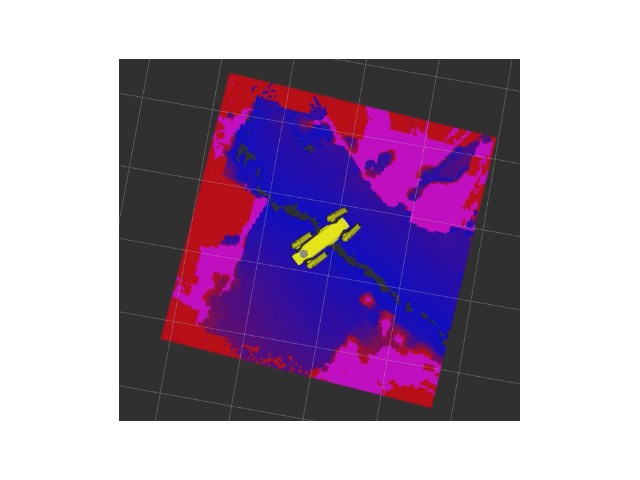
\includegraphics[trim={4cm 3cm 4cm 3.5cm},clip, width=\linewidth]{graphics/costmap_bd2.png}
    \end{subfigure}%
    ~
    \begin{subfigure}{0.5\linewidth}
        \centering
        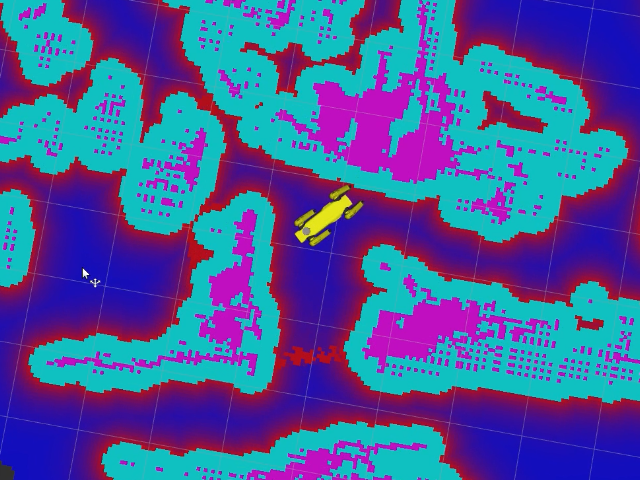
\includegraphics[trim={1cm 1cm 1cm 1cm},clip, width=\linewidth]{graphics/costmap_bd2_embedded.png}
    \end{subfigure}
    \caption{Left:  Risk map generated from Spot's onboard cameras with lethal (pink), high-risk but non lethal (red), and low risk (blue) regions. Right: Au-Spot risk map layer combined with LiDAR based risk map showing larger range of obstacles for a more robust and long-range planning.}
    \label{bd_costmap}
\end{figure}

% \begin{itemize} % For Mission Autonomy(Behavstmap) -> iours, IRM) probably we just gonna cite Scott and Kyon aero paper. 
%         \item Traversability (settling, collision check, slope check, negative obstacles,..) (David?)
%     \item Local Planning (our traversability/local planner complements BD's internal one. We have long range LiDAR, bigger costmaps and detect negative obstacles. In the local planner, we can encourage forward motion in order to avoid walking into the robot's blind spot and increasing the chance of seeing artifacts with the forward facing sensors)
% \end{itemize}

%%%%%%%%%%%%%%%%%%%%%%%%%%%%%%%%%%%%%%%%%%%
\section{Mission planning}\label{sec:mission_planning}
%\inst{not clear if we need this section}
%\todo{Scott-Kyon-FadNik} \ph{Mission and its challenges}

%In the SubT Challenge, robots are expected to rapidly map, navigate, and search unknown underground environments, and report back to the human supervisor at the base station. Particularly,t

The Urban Circuit of the DARPA SubT Challenge presented many challenges to competitors and their autonomous robots. This included complex topology (multiple stories, dead-ends, junctions, narrow corridors and open spaces), mobility challenges (stairs, vertical shafts), and communication mitigating layouts (non-line-of-sight labyrinth) which can result in intermittent communication between collaborative robots and the base station. Our robots are designed to autonomously detect and explore new frontiers, as well as sharing distinctive environmental elements with each other and the base station. To ensure optimal communication and thus frontier advancement in any given environments, Au-Spot can deploy communication nodes.

% \todo{Scott-Amanda-Sung} 
\ph{Behaviors and Modes}
%Hence, t
There are different high-level behaviors in the mission planning layer. 
We denote the behavior library as
\begin{align}
    \mathcal{B} = \{B^1,\cdots,B^n \}
\end{align}
The role of the mission planner is to generate a sequence of behaviors:
\begin{align}
    (B_0,B_1,\cdots,B_T) = \arg\min MissionRisk(\mathcal{B})
\end{align}
A given behavior $B^i$ is executed by (i.e., defined as) visiting a set of anchor points (i.e., nodes) in the information space as explained further below. 

%\todo{Sung-Amanda-David} \ph{IRM}
\ph{Mission Risk}
To quantify the aforementioned mission risk, we first create a sparse graph structure $G = (V, E)$ to capture the connectivity of the free space in the environment. 
We refer to this graph as the IRM (information roadmap) as its nodes ($V$) and edges ($E$) are enriched by various environmental and robot-related properties. As an example, in the Urban Circuit, a node at the entrance of a staircase is marked with a special attribute which indicates that a high level of traversability%, unique to Spot, 
is required to plan paths through this node. 

\ph{Information Roadmap}
IRM nodes are categorized as either breadcrumbs ($\beta\in\mathbb{B}$), frontiers ($f\in F$), or the home base ($h\in H$) where the mission is initiated. 
\begin{align}
    V = (F, \mathbb{B}, H)
\end{align}
Frontier nodes are located at the boundary between unexplored and known space, and are connected to breadcrumb nodes though collision-free edges. %9
Pose graph-fixed breadcrumb nodes trace the history of the robot's motions and, hence, indicate both known areas and traversable paths via breadcrumb edge connections. %4.5
Furthermore, since robots share their pose graph with one another, frontier nodes are never placed in already explored areas.  
%Also, frontier nodes and their edge connections on the IRM encode where the unexplored regions are, how significant they are for the global coverage, and how to traverse to them in this multi-level environment.
%The global planning module provides services to maintain and query the IRM, such as adding/pruning frontier nodes. Behaviors can query the global planner for the shortest path to frontiers, closest stairs, and the base station. Additionally, the planner is responsible for ensuring that the locations of the IRM nodes remains consistent after a pose-graph relaxation from the global localization module.  

% \begin{align}
%     E = (T, D, ...)
% \end{align}

%\todo{Amanda-David-Sung}
\ph{Exploration Planning} 
The objective of the global planning module is to assign frontiers as terminal goals to maximize global coverage of the environment by multiple robots, including the Au-Spots, for the allotted time. Frontier goals are assigned to the robot according to either a local or global selection approach. 
\subsection{Local Frontier Selection}
Given the robot's current pose ($x_k$), we select a frontier goal ($f_g$) with minimum bearing (i.e. relative planar angle between robot's forward direction and frontier location), subject to traversability and bearing constraints:
\begin{align}
    J^{local}(V, E, x_k) &= \theta_{bearing}(x_k, f) 
\end{align}
\begin{align}
    f_g &= \arg\min_{f\in V} J^{local}(V, E, x_k)\\
    ~s.t.,~~~ & P_{travs}(x_k, f) > \gamma \nonumber \\
    % & f \in Disc(x_k, r)\\ NOTE we choose this range so we can make a judgement about traversability, so prob not necessary to make it a separate constraint
    & |\theta_{bearing}(x_k, f)| < \pi/2 \nonumber
\end{align}
$P_{travs}(x_k, f)$ is the probability of a traversal between $x_k$ and $f$. 
While the first constraint ensures that the selected frontier is traversable, the latter constraint on the bearing angle $\theta_{bearing}(x_k, f)$ results in a depth-first exploration behavior. 
Note that for the local frontier selection, the frontiers in the direction of robot's current heading are preferred in order to minimize velocity changes during traversal. This scheme is particularly helpful for Au-Spot so that it can walk continuously at higher speeds and minimize turning motions which may cause risky foot placements at the blind spots (at the rear-left and -right) of the robot.

\subsection{Global Frontier Selection}
Global frontier selection is initiated if no frontier exists satisfying local selection constraints. Frontiers $F$ in the IRM $G$ are clustered according to the minimum number of edges connecting any two sets of observations through a hierarchical agglomerative clustering strategy. A cluster is defined as:
\begin{align}
    % cluster(f) = \{ f' | d(f', f) < n_{E} \}\in\mathcal{C}
    C(f) = \{ f' | dist(f', f) < n_{E} \}\in\mathcal{C} 
\end{align}
Since cluster size is indicative of an unexplored region's expanse, we use it to predict expected information gain, or the utility of traversing to a frontier in that cluster. For a given cluster, the minimum number of edges between the robot's current position and the cluster is the cost of traversal. We select a frontier goal $f_g$ closest to the centroid of the cluster $C_g(f)$ which maximizes our cost-utility function:
\begin{align}
    J^{global}(V, E, x_k) = w_{d}(dist(x_k, f))^{-1} + w_{s}|C(f)|
\end{align}
\begin{align}
    C_g(f) &= \arg\max_{C\in \mathcal{C}} J^{global}(V, E, x_k) \\
    % ~s.t.,~~~ & dist(x_k, C) < \gamma' \nonumber \\
    f_g &= \arg\min_{f\in C_g(f)} dist(f, centroid(C_g(f)))
\end{align}
where $w_d$ and $w_s$ weigh the cost of traversal and new information gain, respectively. 
A robot travels to a global frontier goal $f_g$ by backtracking and planning paths along its breadcrumbs.
% Since the robots share their explored regions with each other, the global planner can automatically deploy them to different sectors of the environment. 
% \begin{align}
%     J(V, E; x_k) = dAng(f, x_k)
% \end{align}

% \begin{align}
%     nextWyapoint &= \arg\min_{f\in V} J(V, E)\\
%     ~s.t.,~~~ & P(f, x_k) > \gamma \\
%     & f \in Disc(x_k, r)\\
%     & dAng(f, x_k) < \zeta
% \end{align}
% \begin{align}
%     cluster(f) = \{ f' | d(f', f) < r \}\in\mathcal{C}
% \end{align}


% \begin{align}
%     J^{global}(V, E; x_k) = w_s |Cluster(f)| + w_d degree(f)
% \end{align}

% \begin{align}
%     C^s &= \arg\max_{c\in \mathcal{C}} J^{global}(V, E)\\
%     ~s.t.,~~~ & d(C, f) < \gamma' \\
% \end{align}

% \begin{align}
%     f^* &= centroid(C^s)
% \end{align}


% \begin{figure}[thpb]
%   \centering
%   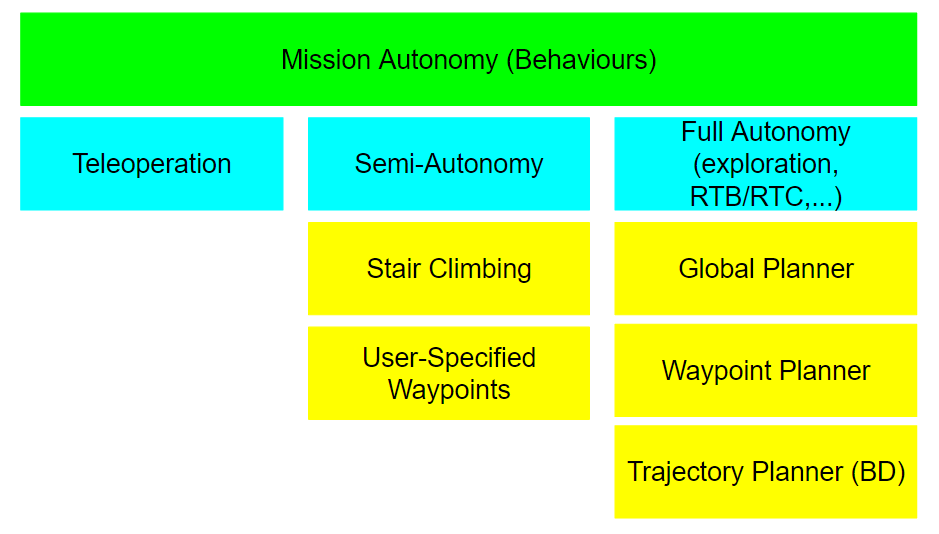
\includegraphics[width=0.40\textwidth]{graphics/spot_planning.PNG}
%   \caption{\inst{not sure if we need this} Planner Architecture on Spot. TODO@Nikhilesh: Make cleaner graphic}
%   \label{figurelabel}
% \end{figure}

% Then, we need to discuss how traversability and risk values (from the previous section) appear on IRM edges... \inst{since we are not doing this yet, this might need some coding or we can remove this section}... similarly, we should show how stairs semantics appear on teh IRM... similarly, we can discuss when the robot calls operator for help (it shoudl be the "result" of planning. for example, when the planning returns a plan which has a risk beyond 70 percent). The output of planning could be from a activity library (e.g., explore, rtb, rtc, teleop, stair climbing,...). This set (activity library) needs to be defined mathematically and the plannign probelm shoudl be formulated as a optimization over this activity library space.


\begin{figure}[t!]
  \centering
  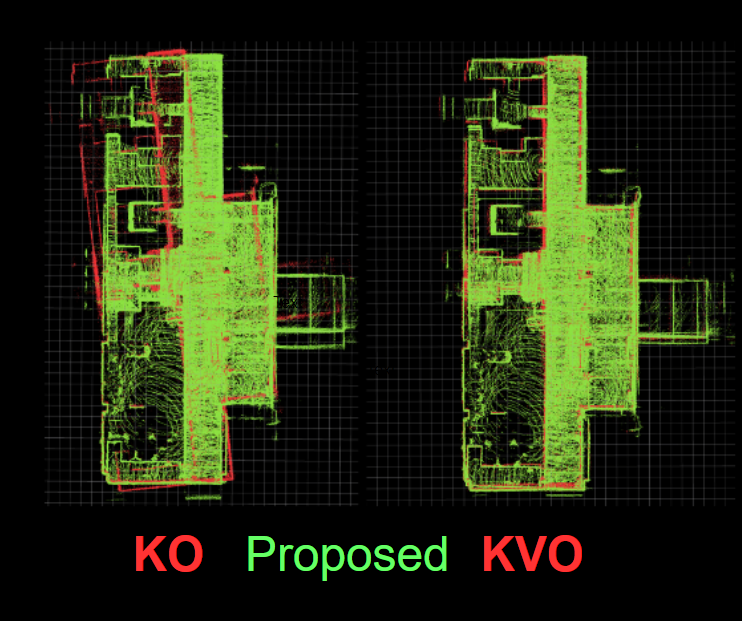
\includegraphics[width=0.47\textwidth]{graphics/spot_proposed_eagle_rock.PNG}
  \caption{Map created by Au-Spot exploration of Eagle Rock Substation, Los Angeles \rev{\st{(CA)}} with different odometry sources: proposed method in green against a) KO and b) KVO}
  \label{spot_eagle_rock}
\end{figure}

\begin{figure}[t!]
  \centering
  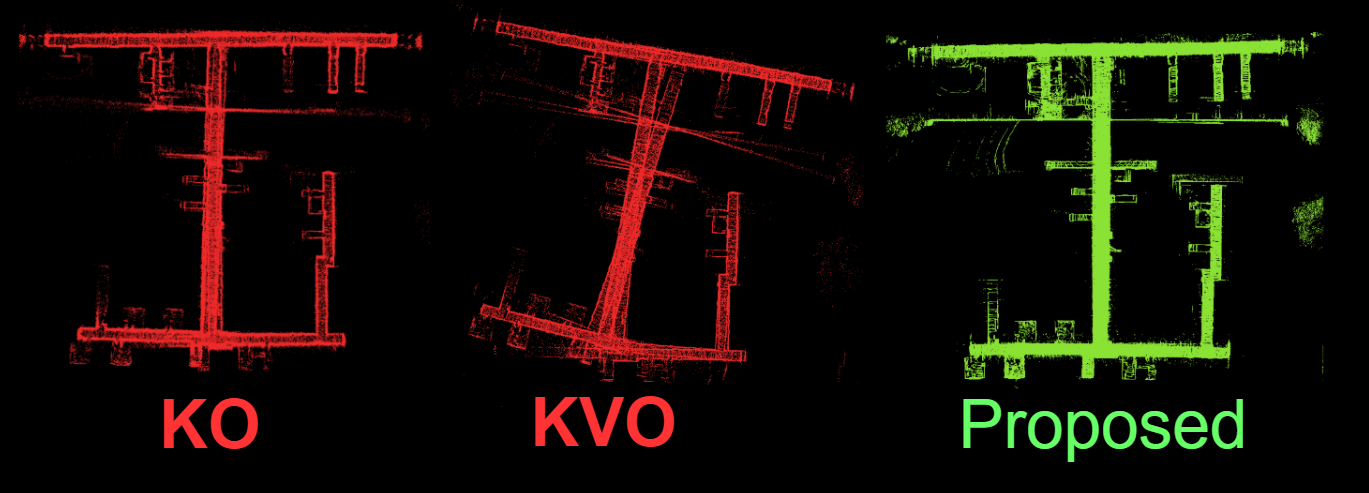
\includegraphics[width=0.47\textwidth]{spot_iros/graphics/spot_proposed_office.PNG}
  \caption{Map created by Au-Spot while exploring an office building at NASA's JPL with different odometry sources: a) KO b) KVO c) Proposed}
  \label{spot_indoor_office}
\end{figure}


\ph{Stair Climbing}
A special case that is not handled by the local planner is stair climbing. 
%\rev{Stairs will either appear as positive or negative obstacles in the risk map.} 
In the current setting, stair climbing is semi-autonomous. The human supervisor has to \rev {\textit(i)} detect the presence of a stair case \rev{(e.g. from the robot Camera/LIDAR feed)}, \rev {\textit(ii)} switch Spot's internal planner to 'Stair' mode which configures the planner for climbing stairs, and then \rev {\textit(iii)} give \rev{a goal} at the end of the stair case. The actual climbing is then completely handled by Spot's internal planner and controller.

%%%%%%%%%%%%%%%%%%%%%%%%%%%%%%%%%%%%%%%%%%%
\section{Experimental Results}\label{sec:experiments}
%%%%%%%%%%%%%%%%%%%%%%%%%%%%%%%%%%%%%%%%%%%

%\todo{everyone}\inst{combine below two paragraphs}
The NeBula autonomy framework is implemented onto two Boston Dynamics Spot robots and has been field-proven in subsurface, multi-level, perceptually degraded and GPS-denied environments, including office buildings, underground buildings and power plants.

As part of the Urban Circuit of the DARPA Subterranean Challenge, two Au-Spots were deployed into the Satsop Power Plant in February 2020 for live-mission exploration and artifact detection e.g. backpacks, gas leaks, human survivors. 
The Au-Spots were able to explore \rev{the plant successfully and accurately report artifact locations back to the human-supervised base station, in real-time.}

%multi-level environments and report back accurate artifact locations to the human supervisor at the base station.

\rev{Both Au-Spots traveled a combined distance of 4km in four runs, including successfully climbing multiple flights of stairs, four times.}
%Specifically, the two traveled a combined distance of 4 km in four runs, including four successful stair climbing of multiple flights of stairs. 
\rev{The Au-Spots successfully detected a total of 25 artifacts across all four runs of Alpha and Beta courses, with the best runs of each course amounting to a grand total of 16 points for our team, CoSTAR.}
%mentioning the sensors is kind of redundant, we have mentioned that that is how they do their detection earlier in the paper and we know that Au-Spot is NeBula enabled. 

\ph{Odometry Estimation}
To demonstrate the performance of the proposed multi-modal odometry pipeline on a legged robot, we evaluate and compare the localization accuracy using individual sensing channels with the proposed uncertainty-aware multi-sensor approach in perceptually-degraded environments. 

Fig. \ref{spot_eagle_rock} depicts the results of the proposed method on data collected in an underground subway station in Eagle Rock, Los Angeles. As seen in this figure, KO performs poorly in this environment whereas KVO results in a reasonably accurate map. %On the other hand, 
Conversely, Fig. \ref{spot_indoor_office} shows the results from the data collected in NASA JPL's 198/161 buildings where KO provides much more accurate maps than KVO. Features of various courses makes the perception and odometry challenging to various sensing channels. 

%As can be seen in these figures, 
\rev{As seen in Fig. \ref{spot_eagle_rock} and Fig. \ref{spot_indoor_office},}the proposed odometry generation method results in consistently more accurate maps than those obtainable by KO or KVO-based odometry. %is computationally light-weight and therefore accounts for the limited computational capability of the on board processing unit.

Finally, the proposed odometry solution was employed by team CoSTAR's Au-Spots at the DARPA Subt Challenge and this resulted in highly accurate maps.

%Finally, the proposed odometry solution has been employed on two Spot robots of the CoSTAR team during the exploration of a dismissed multi-level power plant in Elma, WA at the Urban Circuit of the DARPA SubT Challenge, resulting in highly accurate maps. % and leading to the first place for the CoSTAR team in this challenge. 

\begin{figure}[t!]
  \centering
  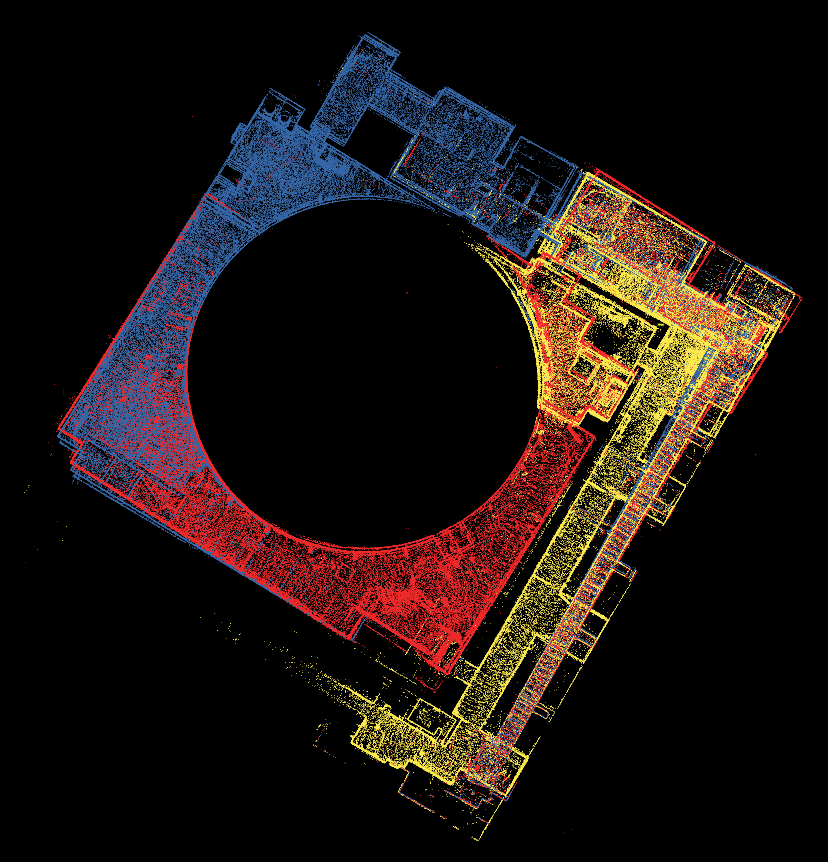
\includegraphics[width=0.4\textwidth]{spot_iros/graphics/coverage_matteo.png}
  %\caption{Area explored by a fleet of two Spots and two wheeled robots.  Colored pointclouds indicate explored areas, with colors indicating z height, spanning 3 floors. (Image credit: DARPA).}
  \caption{\rev{Area explored in the SubT Beta course by a fleet of two UGV's and one Au-Spot. Colors indicate robot-specific coverage (Red: UGV 1, Blue: UGV 2, Yellow: Au-Spot 1).}}
  \label{fig:exploration_planner_topview}
\end{figure}

\begin{figure}[t!]  % Moved from odometry section; Revert if necessary
  \centering
  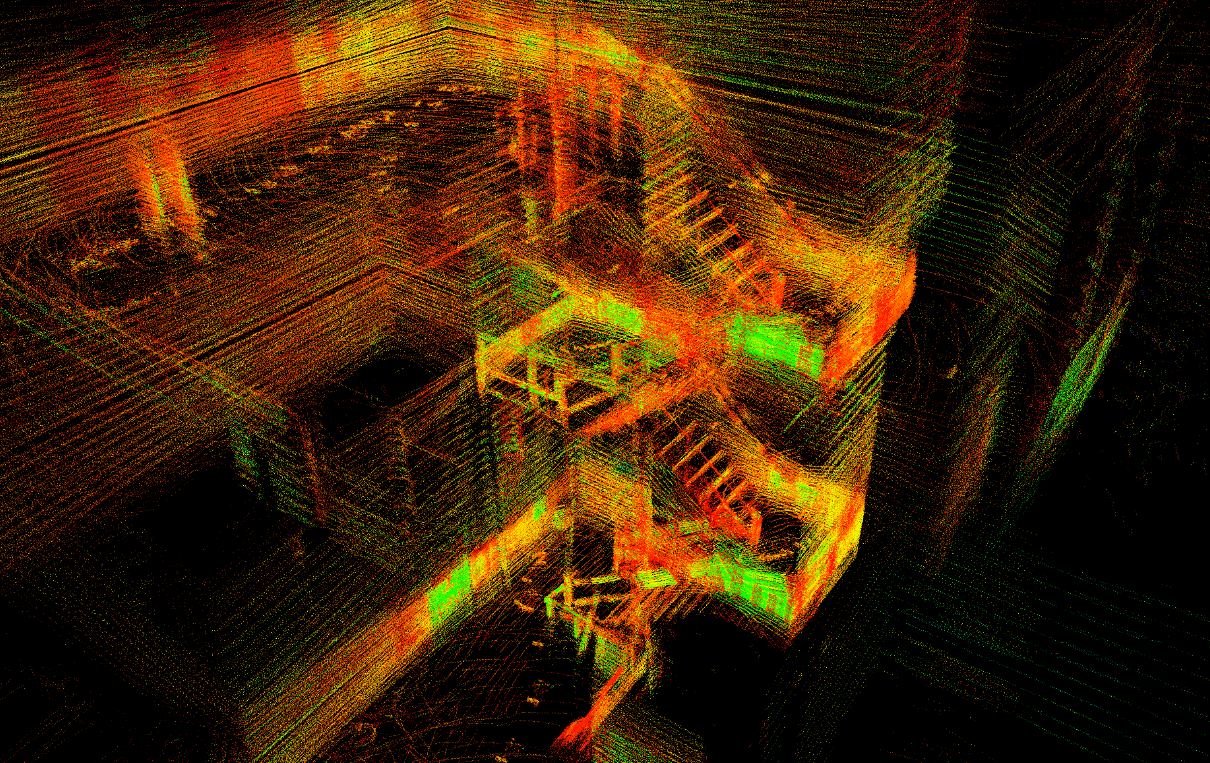
\includegraphics[width=0.45\textwidth]{graphics/spot_alpha_course_stairs.PNG}
  \caption{Map produced with the proposed method in the Alpha Course of DARPA SubT Challenge Urban Circuit.}
  \label{fig:alpha_course_stairs_map}
\end{figure}



% %%%%%%%%%%%%%%%%%%%%%%%%%%%%%%%%%%%%%%%%%%%
% \subsection{Planning and Autonomous Exploration}
% %%%%%%%%%%%%%%%%%%%%%%%%%%%%%%%%%%%%%%%%%%%
\ph{Coverage Planner}
The coverage planner presented in Section \ref{sec:mission_planning} successfully enabled a fleet of two Au-Spots and \rev{two, wheeled UGV robots} to autonomously explore and map the underground environment of an abandoned power plant during the Urban Circuit of the DARPA SubT Challenge. Fig. \ref{fig:exploration_planner_topview} \rev{depicts the area explored by the robots.}

% \begin{figure}[t!]
%   \centering
%   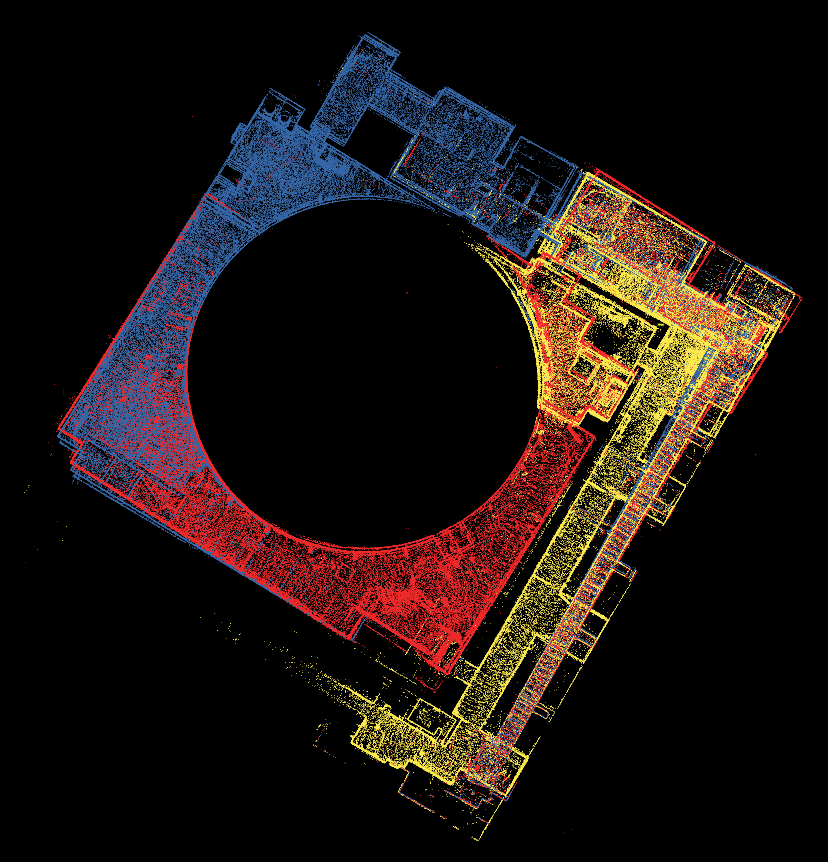
\includegraphics[width=0.45\textwidth]{spot_iros/graphics/coverage_matteo.png}
%   %\caption{Area explored by a fleet of two Spots and two wheeled robots.  Colored pointclouds indicate explored areas, with colors indicating z height, spanning 3 floors. (Image credit: DARPA).}
%   \caption{\rev{Area explored in the SubT Beta course by a fleet of two UGV's and one Au-Spot. Colors indicate robot-specific coverage (Red: UGV 1, Blue: UGV 2, Yellow: Au-Spot 1).}}
%   \label{fig:exploration_planner_topview}
% \end{figure}

% \begin{figure}[t!]  % Moved from odometry section; Revert if necessary
%   \centering
%   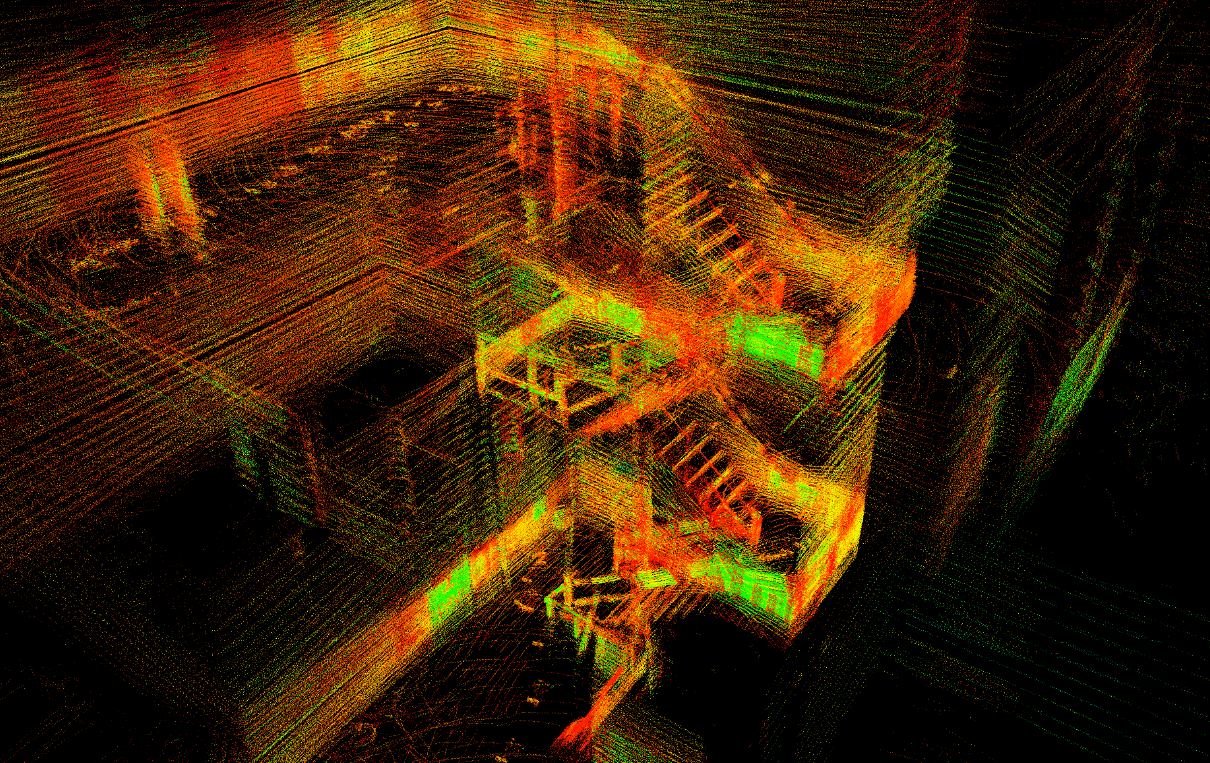
\includegraphics[width=0.45\textwidth]{graphics/spot_alpha_course_stairs.PNG}
%   \caption{Map produced with the proposed method in \rev{the SubT} Alpha Course of DARPA SubT Challenge Urban Circuit}
%   \label{fig:alpha_course_stairs_map}
% \end{figure} % Fadhil moved this above but cannot move the comment


%\textbf{Multi--Level}
%The fully autonomous exploration behaviour, combined with the semi--autonomous stair climbing capability, enabled the Spots to explore multiple levels of the testing facility.
%Fig. \ref{fig:alpha_course_stairs_map} shows the reconstructed map from a multi--level exploration mission.


%\begin{figure}[thpb]
%  \centering
%  \includegraphics[width=0.47\textwidth]{example-image-a}
%  \caption{Exploration on Multiple Levels.}
%  \label{fig:exploration_planner_multilevel}
%\end{figure}

\ph{Traversability}
The traversability analysis module \rev{creates risk maps of size 20mx20m.}
For this, traversability analysis is performed on the map coming from a spatial fusion of LiDAR data with odometry \cite{oleynikova2017voxblox}.
Having a risk map this big is crucial for bridging the gap between Spot's internal planner, which only keeps a robot--centric traversability map in the size of 4x4m, and the goals that are given by the global planner, which can be up to 10 m away from the robot's current position.

Besides seeing further than the internal planner, our traversability analysis, presented in Section \ref{sec:local_planning}, considers metrics such as negative obstacles, sensor blind spots, or dropped comm nodes, which are not considered by the internal planner.
The result was that the Au-Spots were able to successfully avoid negative obstacles, such as stairs going down or avoid planning paths through the sensor blind spots.

% \begin{figure}[thpb]
%   \centering
%     \begin{subfigure}[t]{0.5\linewidth}
%         \centering
%         \includegraphics[height=1in]{example-image-a}
%         \caption{Detecting Positive Obstacles}
%         \label{fig:trav_costmap_pos_obs_wall}
%     \end{subfigure}%
%     ~ 
%     \begin{subfigure}[t]{0.5\linewidth}
%         \centering
%         \includegraphics[height=1in]{example-image-b}
%         \caption{Detecting Negative Obstacles (down stairs)}
%         \label{fig:trav_costmap_neg_obs_stairs}
%     \end{subfigure}
%         \begin{subfigure}[t]{0.5\linewidth}
%         \centering
%         \includegraphics[height=1in]{example-image-a}
%         \caption{Avoiding dropped comm nodes}
%         \label{fig:trav_costmap_comm_nodes}
%     \end{subfigure}%
%     ~ 
%         \begin{subfigure}[t]{0.5\linewidth}
%         \centering
%         \includegraphics[height=1in]{example-image-a}
%         \caption{Avoiding Sensor Blind Spots}
%         \label{trav_costmapb_bd_blindspot}
%     \end{subfigure}%
%     \caption{Traversability Costmaps}
% \end{figure}

\ph{Local Planning}
Our local planner used our bigger traversability map to plan paths to the goals given by the global planner.
As already mentioned, this helped to overcome sub--optimal paths, due to longer planning horizon, and see obstacles, which are not visible to the internal planner.
Additionally, the perception-aware maneuvers as described in Section \ref{sec:local_planning}, helped to bias the robot to move forward.
Because the internal sensors have a blind spot in the rear--left and rear--right and the FoV is better in the front, this succesfully helped to avoid cases, where the robot would step into its blind spots.

% Figure ??? shows the output of the local planner, consisting of the costmap, the A* path and the selected waypoint with the heading, which biases the robot to move forward.
% \begin{figure}[thpb]
%   \centering
%   \includegraphics[width=0.47\textwidth]{example-image-a}
%   \caption{Long--Range Costmap + Dijkstrapath + Waypoint}
%   \label{fig:local_planner}
% \end{figure}

% \begin{figure}[thpb]
%   \centering
%   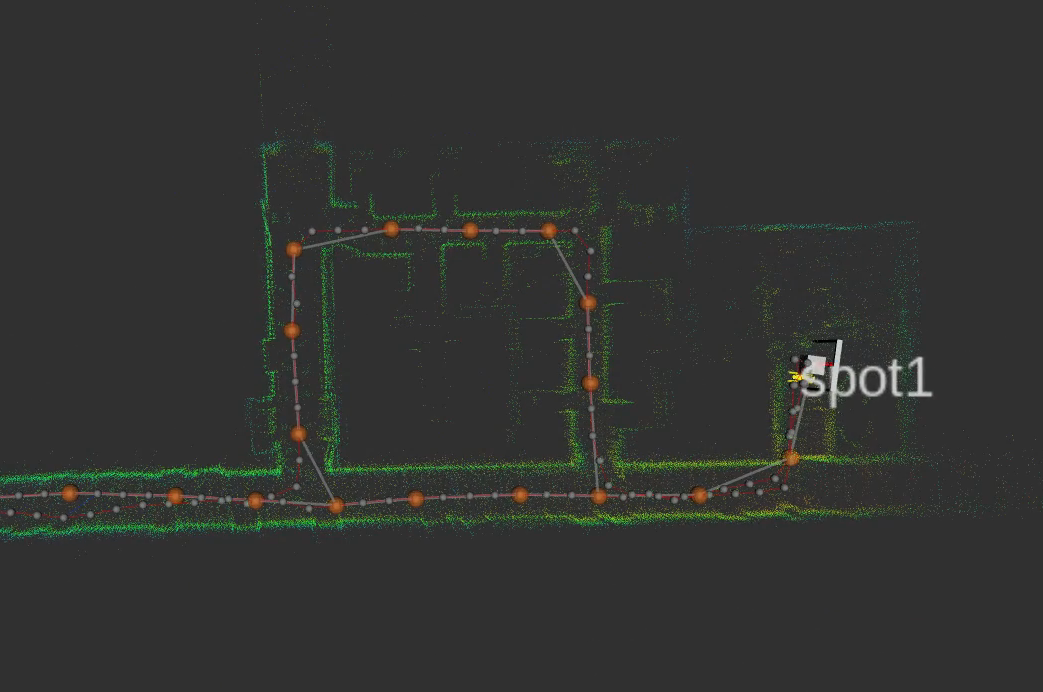
\includegraphics[width=0.4\textwidth]{graphics/irm.png}
%   \caption{IRM constructed while exploring a single level.}
%   \label{figurelabel}
% \end{figure}


%%%%%%%%%%%%%%%%%%%%%%%%%%%%%%%%%%%%%%%%%%%
\ph{Stair Climbing and Multi-level Mapping}
%%%%%%%%%%%%%%%%%%%%%%%%%%%%%%%%%%%%%%%%%%%
\rev{As previously mentioned, Au-Spot successfully climbed multiple flights of stairs during the Urban Circuit of the DARPA Subterranean Challenge.}
%demonstrated four successful stair climbing during the Urban Circuit scored runs. 
Each staircase consists of four flights of stairs with tight 180-degree turns at each landing. 
The stairs are metal-grated and approximately 0.27m in run, and 0.19m in rise. Fig. \ref{fig:stairs-firstPage} shows a snapshot of \rev{Au-Spot in the Alpha course, successfully climbing down stairs.} 
Stair climbing operations pose challenges to state estimation due to the frequent pitching motion, physical slippages on the stair edges, and repetitive patterns of the railing. 
Fig. \ref{fig:alpha_course_stairs_map} is the map produced during the stair climbing operations, which led to high-precision localization of artifacts ($\leq$ 5 m error).


% \begin{figure}[t]
%   \centering
%   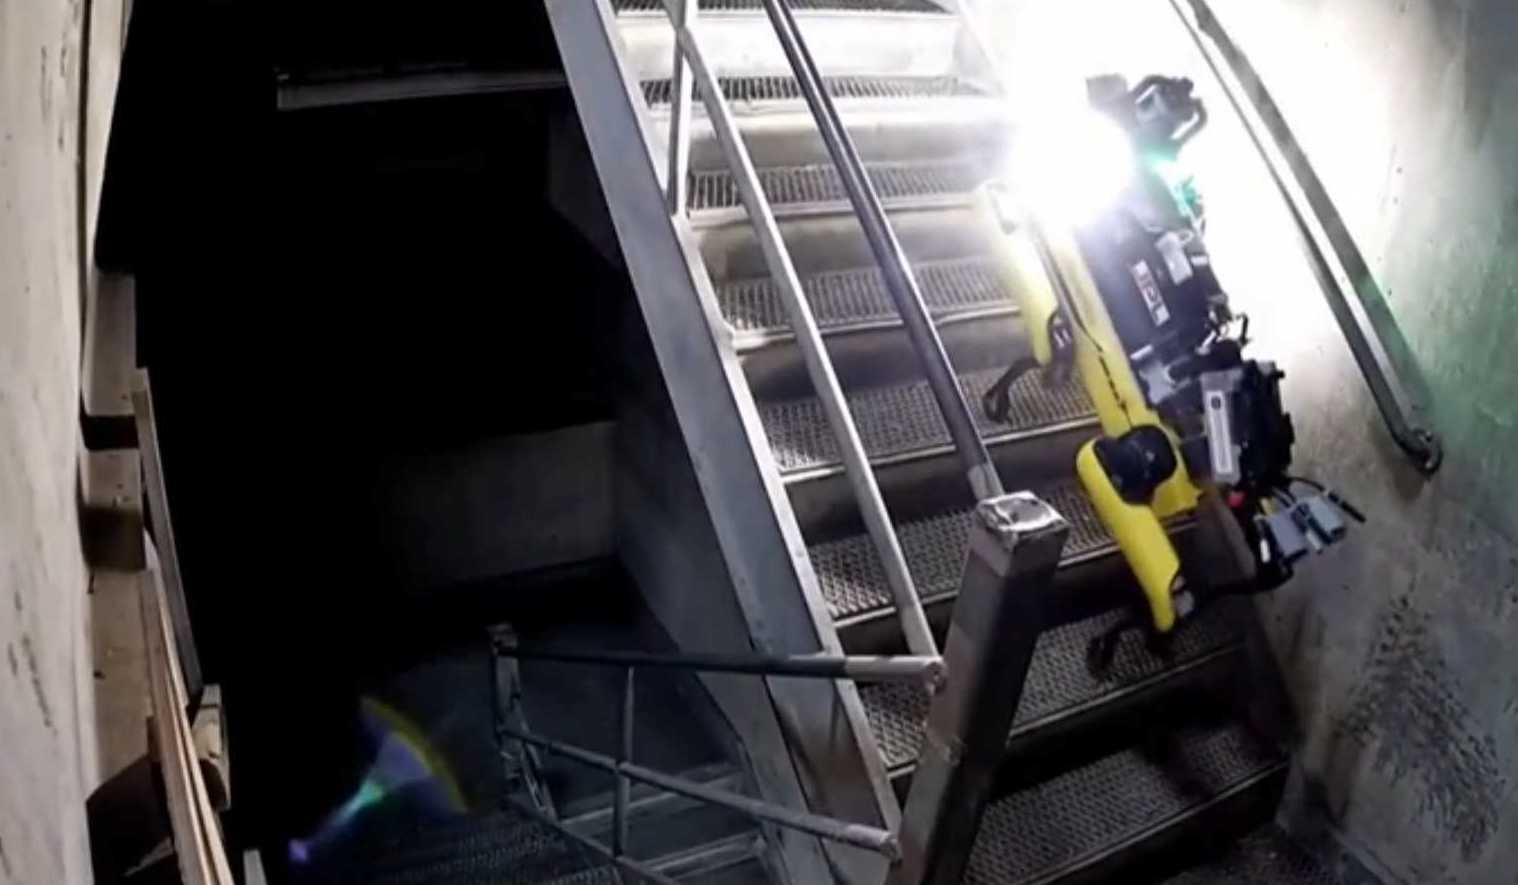
\includegraphics[width=0.45\textwidth]{graphics/spot_stairclimbing2.jpg}
%   \caption{Spot stair climbing in Urban Circuit Alpha course.}
%   \label{fig:spot_stair_climb}
% \end{figure}

\begin{figure}[thpb]
  \centering
  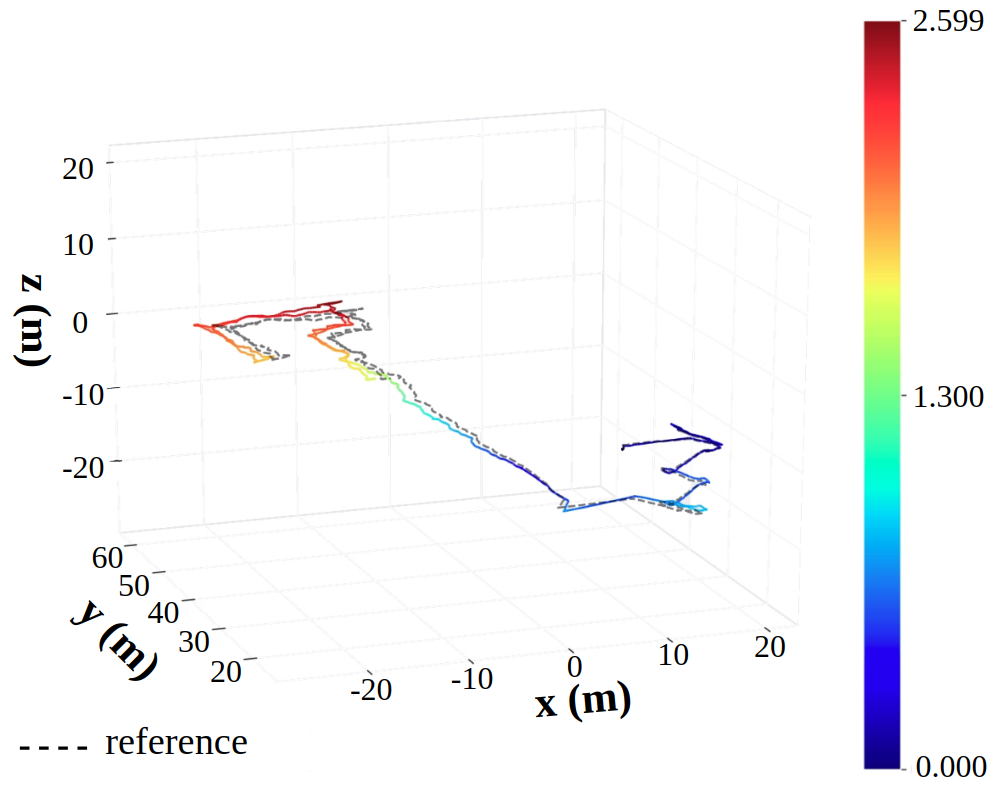
\includegraphics[width=0.47\textwidth]{spot_iros/graphics/spot2_alpha2_ape.png}
  \caption{\rev{Absolute Position Error (APE) of Au-Spot 2 in Alpha 2 course. TODO: To be linked with text}}
  \label{spot2_alpha2_ape}
\end{figure}

% %%%%%%%%%%%%%%%%%%%%%%%%%%%%%%%%%%%%%%%%%%%
% \subsection{Spot Operation in DARPA SubT Urban Circuit}
% %%%%%%%%%%%%%%%%%%%%%%%%%%%%%%%%%%%%%%%%%%%
% \inst{Lots of amazing pictures, accuracy of localization, traversability
% Images of: Spot in extreme terrain, LAMP Map, IRM, Comms map, Comm dropping, Stair Climbing}

% \newpage

% %%%%%%%%%%%%%%%%%%%%%%%%%%%%%%%%%%%%%%%%%%%
% \section{Lessons Learned and Future 
% Directions}\label{sec:lessonslearned}
%%%%%%%%%%%%%%%%%%%%%%%%%%%%%%%%%%%%%%%%%%%
% Robosimian's journal intro sentences of lessons learned
% This section summarizes some of the highlights of our platform,
% discusses the lessons learned, and justifies the core
% assumptions we made in design, testing, and operations:
% % I think its not in order yet

% % Fadhil. May be this subsection can be moved to Robot behaviors?
% \subsection{Recovery}
% Due to the challenging terrain of Spot at the test area, we consider a possibility that the robot might fall.
% %
% Fortunately, Spot has ability to "SELFRIGHT" itself from falling to sitting position and still operational after that.
% %
% However, on some cases, we find that the robot is not able to stand up after a successful "SELFRIGHT" because the legs placement are not stable after the recovery.
% %
% As a work around to robustify the behaviors in the current Spot software that we use, we send a repetitive command of quick stand and sit to improve better placement of the legs.

% \subsection{Traversability}
% Currently, traversability is purely defined geometrically (obstacles, slopes, holes,...).
% However, when traversing challenging terrains, as encountered in the SubT challenge, the notion of traversability has to be extended.
% While there are many metrics, which can be considered for traversability and that have been described by Papadakis in \cite{Papadakis2013}, the most important one would be surface friction.
% Due to small contact surface and, compared to wheeled or tracked robots, and dynamic gaits, quadrupeds suffer more from slippery surfaces such as wet or dusty surfaces. 

% For this reason, traversability has to include surface friction informations so that it can be avoided by the local planner, if possible.
% If avoidance should not be possible, this information could at least be used to adaptively set the surface friction coefficient, which is used by the Spot's internal planner.

% Another traversability metric might include terramechanics in order to avoid soft soil, where the feet of the robot might sink in.

% Another traversability metric might be to not step on movable items (loose plates or things on which Spot crashed)

% => We need traversability from semantic scene understanding, not just geometric anymore!!!

% \inst{This kind of discussion should go to the experiment section. - This does not fit the method section} The Nebula global planner, which is described in more detail in Section \ref{sec:mission_planning}, can select goals up to 10 m away from the current robot's position.
% However, Spot's internal planner works with a 4x4 m map of the environment.
% Even though, waypoints outside of the internal map can be given to the internal planner, this caused some issues such as the robot taking sub--optimal paths or not avoiding some obstacles such as overhangs, cliffs or obstacles within the blind spots of the internal sensors.
% Because, the Nebula payload offers more sensing capabilities, especially due to the long--range sensors such as the LiDAR, we chose to add an intermediate planner in order to bridge the gap and avoid and complement the Spot internal planner.

% ======

% \subsection{Perception--Aware Planning}
% Legged robots, such as Spot, have a higher degree--of--freedom than most ground robots, which usually have a fixed chassis.
% This higher level of configurability decouples the robot's overall motion from the floating base's attitude to a certain extent.
% One interesting direction would be to exploit this characteristic of the floating base for perception--aware planning.
% For example by pitching or rolling the robot's base in order to maximize sensor coverage and reduce blind spots.

% ====

% We have access to BD costmap and additional obstacle information, which spot might not see. When giving global waypoints (far away), the robot might not be able to avoid some of these or end up taking suboptimal paths due to the small costmap (4x4m). We plan intermediate waypoints (with Dijkstra) to avoid this problem. Additionally, we prefer forward motion due to sensor coverage (blind spot avoidance and artifact detection), so we choose the waypoint heading in a way which encourages the robot to go forward. Waypoints are given to Spot's internal planner, which then executes the actual trajectory.

% Mentio that, even though we can try to avoid these regions by not giving waypoints in that region we cannot guarantee that BD will actually avoid these regions.

% Define, how we assign an orientation to the previously selected waypoint in order to bias forward motion


% \subsection{Intelligent Behaviour Selection}
% Automatics stair detection and climbing, changing gaits (crawl) to get over rubble,...)
% BD offers a very limited, but powerful, set of tuning knobs (gait, stair mode, surface friction, body height,...).
% However, these are either set to fixed average values or chosen by the human supervisor.
% One push would be to switch and set these tuning knobs autonomously (for example choose gait based on what the long range sensors see, set surface friction by estimating surface friction, autonomously change to stair mode and do autonomous stair climbing instead of human given wp)


% \subsection{Collaboration}
% Spot as drone carrier?
%%%%%%%%%%%%%%%%%%%%%%%%%%%%%%%%%%%%%%%%%%%
\section{Conclusions}\label{sec:conclusions}

\rev{This system-focused paper reports our work on endowing the Boston Dynamics Spot robot with high-levels of autonomy, hardware and perception capabilities that won the Urban Circuit of the DARPA Subterranean Challenge.}
%This system-focused paper reports our work on endowing high-level autonomy and perception capabilities on the Boston Dynamics Spot robot that won the Urban Circuit of the DARPA Subterranean (SubT) Challenge. 
In this paper, \rev{we briefly discussed our NeBula autonomy architecture which we augmented to Boston Dynamics' Spot and described specific aspects to enabling legged autonomy in complex missions.}  
% and explained in more detail the odometry and risk-aware planning aspects of the autonomy framework. 
We believe this work is an important step in demonstrating the capabilities of legged robots to accomplish complex real-world missions in extreme environments.

%Motivated by exploring extreme environments and in particular underground environments in DARPA SubTerranean Challenge, this paper pushes the boundaries of the state-of-practice in enabling legged robotic systems to accomplish real-world complex missions in relevant scenarios. In particular, we will discuss the behaviors and capabilities which emerge from the integration of the autonomy framework NeBula (Networked Belief-aware Perceptual Autonomy) with next generation mobility systems. We will discuss the design, hardware, software challenges and solutions in mobility, perception, autonomy, and wireless networking, as well as lessons learned and future directions. We demonstrate the performance of the proposed system and solutions on physical systems in real-world scenarios, which achieved first place in the 2020 DARPA Subterranean Challenge Urban Circuit.


%%%%%%%%%%%%%%%%%%%%%%%%%%%%%%%%%%%%%%%%%%%



\addtolength{\textheight}{-12cm}   % This command serves to balance the column lengths
                                  % on the last page of the document manually. It shortens
                                  % the textheight of the last page by a suitable amount.
                                  % This command does not take effect until the next page
                                  % so it should come on the page before the last. Make
                                  % sure that you do not shorten the textheight too much.

%%%%%%%%%%%%%%%%%%%%%%%%%%%%%%%%%%%%%%%%%%%%%%%%%%%%%%%%%%%%%%%%%%%%%%%%%%%%%%%%



%%%%%%%%%%%%%%%%%%%%%%%%%%%%%%%%%%%%%%%%%%%%%%%%%%%%%%%%%%%%%%%%%%%%%%%%%%%%%%%%



%%%%%%%%%%%%%%%%%%%%%%%%%%%%%%%%%%%%%%%%%%%%%%%%%%%%%%%%%%%%%%%%%%%%%%%%%%%%%%%%
% \section*{APPENDIX}
% A video of the experimental results is available at
% \url{https://youtu.be/_HpWIhFFD54} . \inst{Too dramatic to put on a paper?. Should we put it below abstract?}


% \section*{ACKNOWLEDGMENT}
% The research was carried out at the Jet Propulsion Laboratory, California Institute of Technology, under a contract with the National Aeronautics and Space Administration. This work was partially funded by the Defense Advanced Research Projects Agency (DARPA). Government Sponsorship acknowledged.



%%%%%%%%%%%%%%%%%%%%%%%%%%%%%%%%%%%%%%%%%%%%%%%%%%%%%%%%%%%%%%%%%%%%%%%%%%%%%%%%

%%%%%%%%%%%%%%%%%%%%%%%%%%%%%%%%%%%%%%%%%%%
%%%%%%%%%%%%%%%%%%%%%%%%%%%%%%%%%%%%%%%%%%%
\bibliographystyle{IEEEtran}
\bibliography{main}
%%%%%%%%%%%%%%%%%%%%%%%%%%%%%%%%%%%%%%%%%%%
\end{document}































%------------Review Highlights ---------------------

% Before GENERAL, then ODOMETRY-ORIENTED 

% Environment-INDUCED and Motion-INDUCED Challenges

% 1- One of the main focuses of this work is to enable autonomy in perceptually-degraded environments.

% 2 - This includes ... gps-denied, dark, obscurantc.... This elements pose significant difficulties on various ?sensing modalities?

% 3 - Further, strong platform vibration originated by mobility-stressing terrains exacerbates sensor measurments quality while adding additional uncertainty on sensor measurements (and introduces additional uncertainty on sensor measurements).

% 4 - A reliable odometry source in perceptually-degraded settings is a challenge. %4 --- TODO: Make Better

% A reliable odometry source in perceptually-degraded settings is a challenge. %4 --- TODO: Make Better -  % Motion-induced Challenges

% To overcome these challenges, NeBula characterizes uncertainty and failure modes associated with each sensing modality and formulates a 

% To address these challenges, NeBula relies on a multi-sensor solution to enable odometry in perceptually-degraded setting. Characterizing uncertainty associated and failure modes associated with each sensing modality, NeBula and fuses various sensing modalities in an uncertainty-aware manner

% with health monitor and switch-on-failure capability, that at every time step $k$, selects the odometry channel with the most reliable output transformation $T_k \in SE(3)$.

% motion-prior OR prior INSTEAD of external - Just calling it Y - OK + OR T_init

%---------------------------------------------------------
\comment{SUMMARY: We denote with $L_{k}$ the LiDAR scan collected at time $k$ and with $L_{k-1}$ the LiDAR scan collected at time $k-1$. We indicate with $\textbf{E}^{k-1}_{k} = \textbf{Y}^{-1}_{k-1}\textbf{Y}_k\in SE(3)$ the rigid body transformation of HeRO's output between two consecutive LiDAR acquisitions where, in order to address asynchronous odometry measurements, we interpolate the buffered $\textbf{Y}$ at LiDAR timestamps to $t_{k-1}$, and $t_k$ to get $\textbf{Y}_{k-1}$ and $\textbf{Y}_{k}$: the pose of the HeRO's output at times $t_{k-1}$ and $t_k$, respectively.}